\documentclass[12pt]{amsart}

% ============================================================
% Basic spacing
% ============================================================
\setlength{\lineskip}{0pt}

% ============================================================
% Packages for mathematics
% ============================================================
\PassOptionsToPackage{no-math}{fontspec}
\usepackage{luatexja}
\usepackage[haranoaji]{luatexja-preset}
\usepackage{amsmath}
\usepackage{mathtools}
\usepackage{amssymb}
\usepackage{amsthm}
\usepackage{amscd}
\usepackage{mathrsfs}
\providecommand{\mathds}[1]{\mathbb{#1}} % unused dsfont dependency removed
% unused bbm dependency removed

% ============================================================
% Graphics
% Use the following line for pLaTeX/upLaTeX + dvipdfmx.
% If you compile with pdfLaTeX or LuaLaTeX, remove the option [dvipdfmx].
% For PNG/JPG files with dvipdfmx, run extractbb if LaTeX cannot find the bounding box.
% ============================================================
%\usepackage[dvipdfmx]{graphicx}
\usepackage{graphicx} % Use this instead for pdfLaTeX or LuaLaTeX.

% ============================================================
% Packages for colors and text decorations
% ============================================================
\usepackage[dvipsnames]{xcolor}
\usepackage[normalem]{ulem}
\usepackage{comment}

% ============================================================
% Packages for tables, lists, and diagrams
% ============================================================
\usepackage{multirow}
\usepackage{bigdelim}
\usepackage{enumerate}
\usepackage{enumitem}
% Unused Xy-pic package omitted for native LuaLaTeX compatibility.
\usepackage{tikz}





% ============================================================
% tcolorbox settings
% Use as: \begin{tcolorbox}[mybox] ... \end{tcolorbox}
% ============================================================
\usepackage[most]{tcolorbox}
\tcbuselibrary{breakable, skins, theorems}
\tcbset{
  mybox/.style={
    colback=white,
    colframe=green!35!black,
    fonttitle=\bfseries,
    breakable=true
  }
}



% ============================================================
% Draft tools
% Comment out showkeys before submitting to a journal or arXiv.
% ============================================================
\usepackage[final]{showkeys} % Use this when you want to hide all labels.
%\usepackage{showkeys} % Use this when you want to show labels.
\renewcommand*{\showkeyslabelformat}[1]{%
  \begingroup
  \fboxsep=2pt%
  \fboxrule=0.3pt%
  \fbox{%
    \parbox{1.8cm}{%
      \raggedright
      \normalfont\tiny\sffamily
      \strut #1\strut
    }%
  }%
  \endgroup
}
%

% ============================================================
% This setting makes every enumerate environment use labels of the form (1), (2), (3), ...
% ============================================================


\setlist[enumerate]{label=$(\arabic*)$}

% ============================================================
% Hyperlinks
% Load hyperref near the end of the package list.
% Use the first line for pLaTeX/upLaTeX + dvipdfmx.
% If you compile with pdfLaTeX or LuaLaTeX, use the second line instead.
% ============================================================
%\usepackage[dvipdfmx,colorlinks,linkcolor=red,anchorcolor=blue,citecolor=blue]{hyperref}
\usepackage[colorlinks,linkcolor=red,anchorcolor=blue,citecolor=blue]{hyperref}



% ============================================================
% Page layout
% ============================================================
\setlength{\topmargin}{-0.25cm}
\setlength{\textwidth}{15cm}
\setlength{\textheight}{22.6cm}
\setlength{\headheight}{1em}
\setlength{\headsep}{0.5cm}
\setlength{\oddsidemargin}{0.40cm}
\setlength{\evensidemargin}{0.40cm}
\setlength{\baselineskip}{15pt}
\setlength{\footskip}{32pt}

% ============================================================
% Theorem environments
% ============================================================
\newtheorem{thm}{Theorem}[section]
\newtheorem{theo}[thm]{Theorem}
\newtheorem{cor}[thm]{Corollary}
\newtheorem{prop}[thm]{Proposition}
\newtheorem{conj}[thm]{Conjecture}
\newtheorem*{mainthm}{Theorem}

\newtheorem{deflem}[thm]{Definition-Lemma}
\newtheorem{lem}[thm]{Lemma}

\theoremstyle{definition}
\newtheorem{defn}[thm]{Definition}
\newtheorem{propdefn}[thm]{Proposition-Definition}
\newtheorem{lemdefn}[thm]{Lemma-Definition}
\newtheorem{thmdefn}[thm]{Theorem-Definition}
\newtheorem{eg}[thm]{Example}
\newtheorem{ex}[thm]{Example}
\newtheorem{exa}[thm]{Example}
\newtheorem{ques}[thm]{Question}
\newtheorem{remin}[thm]{Reminder}

\theoremstyle{remark}
\newtheorem{rem}[thm]{Remark}
\newtheorem{setup}[thm]{Setup}
\newtheorem{obs}[thm]{Observation}
\newtheorem{notation}[thm]{Notation}
\newtheorem{claim}[thm]{Claim}
\newtheorem{assup}[thm]{Assumption}
\newtheorem{cln}[thm]{Claim}

% Independent theorem-like environments.
\newtheorem{cl}{Claim}
\newtheorem{step}{Step}
\newtheorem{case}{Case}

% Unnumbered theorem-like environments.
\newtheorem*{clproof}{Proof of Claim}
\newtheorem*{ack}{Acknowledgements}

% Number equations by section.
\numberwithin{equation}{section}

% ============================================================
% Mathematical operators
% ============================================================
\newcommand{\rk}{\operatorname{rk}}
\newcommand{\rank}{\operatorname{rank}}
\newcommand{\degree}{\operatorname{deg}}
\newcommand{\codim}{\operatorname{codim}}
\newcommand{\nd}{\operatorname{nd}}

\newcommand{\Supp}{\operatorname{Supp}}
\newcommand{\supp}{\operatorname{Supp}}
\newcommand{\Rad}{\operatorname{Rad}}
\newcommand{\Exc}{\operatorname{Exc}}
\newcommand{\Div}{\operatorname{div}}

\newcommand{\End}{\operatorname{End}}
\newcommand{\eend}{\operatorname{End}}
\newcommand{\Coker}{\operatorname{Coker}}
\newcommand{\GL}{\operatorname{GL}}

\newcommand{\Hom}{\mathscr{H}\!\mathit{om}}
\newcommand{\SheafHom}[1]{\mathscr{H}\!\mathit{om}_{#1}}
\newcommand{\PGL}{\mathbb{P}\GL(r,\C)}

\DeclareMathOperator{\Ric}{Ric}
\DeclareMathOperator{\Vol}{Vol}
\DeclareMathOperator{\tr}{tr}
\DeclareMathOperator{\Id}{Id}
\DeclareMathOperator{\res}{res}
\DeclareMathOperator{\length}{length}
\DeclareMathOperator{\Homop}{Hom}
\DeclareMathOperator{\Diff}{Diff}
\DeclareMathOperator{\Lie}{Lie}
\DeclareMathOperator{\Autop}{Aut}
\DeclareMathOperator{\Kerop}{Ker}
\DeclareMathOperator{\Imageop}{Im}


% Additional mathematical macros retained from the template 

\newcommand{\MY}{\operatorname{MY}}
\newcommand{\abs}[1]{\left\lvert#1\right\rvert}
\newcommand{\norm}[1]{\left\|#1\right\|} 
\newcommand{\Rm}{\operatorname{Rm}}
\newcommand{\Cal}{\operatorname{Cal}}
\newcommand{\NA}{\operatorname{NA}}

\newcommand{\cA}{\mathcal{A}}
\newcommand{\cB}{\mathcal{B}}
\newcommand{\cC}{\mathcal{C}}
\newcommand{\cD}{\mathcal{D}}
\newcommand{\cE}{\mathcal{E}}
\newcommand{\cF}{\mathcal{F}}
\newcommand{\cG}{\mathcal{G}}
\newcommand{\cH}{\mathcal{H}}
\newcommand{\cI}{\mathcal{I}}
\newcommand{\cJ}{\mathcal{J}}
\newcommand{\cK}{\mathcal{K}}
\newcommand{\cL}{\mathcal{L}}
\newcommand{\cM}{\mathcal{M}}
\newcommand{\cN}{\mathcal{N}}
\newcommand{\cO}{\mathcal{O}}
\newcommand{\cP}{\mathcal{P}}
\newcommand{\cQ}{\mathcal{Q}}
\newcommand{\cR}{\mathcal{R}}
\newcommand{\cS}{\mathcal{S}}
\newcommand{\cT}{\mathcal{T}}
\newcommand{\cU}{\mathcal{U}}
\newcommand{\cW}{\mathcal{W}}
\newcommand{\cX}{\mathcal{X}}
\newcommand{\cY}{\mathcal{Y}}
\newcommand{\cZ}{\mathcal{Z}}

% ============================================================
% Standard maps and geometric notation
% ============================================================
\DeclareMathOperator{\pr}{pr}
\DeclareMathOperator{\id}{id}
\DeclareMathOperator{\Sym}{Sym}

\DeclareMathOperator{\Alb}{Alb}
\newcommand{\verti}{\mathrm{vert}}
\newcommand{\hor}{\mathrm{hor}}
\newcommand{\univ}{\mathrm{univ}}
\newcommand{\reg}{\mathrm{reg}}
\newcommand{\sing}{\mathrm{sing}}
\newcommand{\qt}{\mathrm{qt}}
\newcommand{\can}{\mathrm{can}}
\newcommand{\loc}{\mathrm{loc}}

\newcommand{\orb}{\mathrm{orb}}
\DeclareMathOperator{\tor}{Tor}
\newcommand{\Tor}{\mathrm{tor}}

\newcommand{\Sha}{\operatorname{Sha}}
\newcommand{\sha}{\operatorname{sha}}
\newcommand{\Shaf}{\mathrm{Sha}}
\newcommand{\shaf}{\mathrm{sha}}

% ============================================================
% Differential-geometric notation
% ============================================================
\newcommand{\ddbar}{\frac{\sqrt{-1}}{2\pi} \partial \bar{\partial}}
\newcommand{\deldel}{\sqrt{-1}\partial \overline{\partial}}
\newcommand{\dbar}{\overline{\partial}}

\newcommand{\pdrv}[2]{\frac{\partial #1}{\partial #2}}
\newcommand{\drv}[2]{\frac{d #1}{d#2}}
\newcommand{\ppdrv}[3]{\frac{\partial #1}{\partial #2 \partial #3}}

\newcommand{\polar}{\Omega}

% ============================================================
% Sheaves, ideals, automorphisms, kernels, and images
% ============================================================
\newcommand{\sO}{\mathcal{O}}
\newcommand{\mO}{\mathcal{O}}
\newcommand{\cV}{\mathcal{V}}
\newcommand{\I}[1]{\mathcal{I}(#1)}
\newcommand{\Aut}[1]{\Autop(#1)}
\newcommand{\Ker}[1]{\Kerop(#1)}
\newcommand{\Image}[1]{\Imageop(#1)}

% ============================================================
% Number systems and standard spaces
% ============================================================
\newcommand{\R}{\mathbb{R}}
\newcommand{\Z}{\mathbb{Z}}
\newcommand{\N}{\mathbb{N}}
\newcommand{\C}{\mathbb{C}}
\newcommand{\Q}{\mathbb{Q}}
\newcommand{\D}{\mathbb{D}}
\newcommand{\mP}{\mathbb{P}}
\newcommand{\B}{\mathds{B}}
\newcommand{\T}{\mathbb{T}}
\newcommand{\G}{\mathbb{G}}

% ============================================================
% Chern character, Todd class, Chow groups, and volumes
% ============================================================
\DeclareMathOperator{\ch}{ch}
\DeclareMathOperator{\td}{td}
\DeclareMathOperator{\Td}{Td}
\DeclareMathOperator{\CH}{CH}
\DeclareMathOperator{\vol}{vol}
\DeclareMathOperator{\Amp}{Amp}
\DeclareMathOperator{\Cone}{Cone}
\newcommand{\dR}{\mathrm{dR}}

% ============================================================
% Special symbols and formatting shortcuts
% ============================================================
%\newcommand{\tl}{\hspace{-0.8ex}<\hspace{-0.8ex}}
%\newcommand{\tr}{\hspace{-0.8ex}>}

\newcommand{\xb}[1]{\textcolor{blue}{#1}}
\newcommand{\xr}[1]{\textcolor{red}{#1}}
\newcommand{\xm}[1]{\textcolor{magenta}{#1}}

% This command places a short explanation below an equality or inequality sign.
% Example: A \underalign{\text{by Lemma 1.1}}{=} B.
\newcommand{\underalign}[2]{\quad \underset{\mathclap{\strut #1}}{#2}\quad}



\usepackage{booktabs,longtable,array,listings,needspace}
\lstset{basicstyle=\ttfamily\scriptsize,breaklines=true,columns=fullflexible,keepspaces=true,showstringspaces=false}
\setlength{\emergencystretch}{2em}
\newcommand{\Package}{\mathcal F}
\newcommand{\revpol}[1]{#1^{\vee}}
\newcommand{\sg}{\operatorname{sg}}
\newcommand{\ctype}{\operatorname{type}}
\newcommand{\Jin}{J_{\mathrm{in}}}
\newcommand{\Jout}{J_{\mathrm{out}}}
\newcommand{\clK}[1]{\widehat{#1}}
\newcommand{\eps}{\varepsilon}
\newcommand{\RR}{\mathsf R}
\newcommand{\TT}{\mathsf T}
\title[Sharp separation for long virtual knots]{Sharp separation from twelve intersection polynomials:\\
long virtual knots with identical closures}
\author{chatGPT 6Astra}
\date{September 10, 2026}
\subjclass[2020]{Primary 57K12; Secondary 57K14, 57K16}
\keywords{long virtual knot, intersection polynomial, Gauss diagram, exact enumeration, based matrix, separation}
\begin{document}
\begin{abstract}
We determine the least crossing bound for separation by the Satoh--Wada
polynomials from the full twelve-polynomial intersection package: it is two.
If both degree-two GPV invariants and the entire oriented closure must also
agree, the least bound is three. An explicit family on the flat strings
$\alpha_{2m,2m}$ has identical closures and identical intersection packages,
whereas its two $V$-polynomials are
$-t^{m+1}(1+t+\cdots+t^{m-1})^2$ and those of its partner are obtained by
$t\mapsto t^{-1}$. We give all twelve closed formulas, prove crossing number
$4m$ and supporting genus two, and prove that the Jones polynomial is one.
An unreduced enumeration through four crossings and two exact implementations
provide reproducible checks. The novelty claim concerns these joint separation
statements, not the pre-existing invariants or flat strings.
\end{abstract}
\maketitle
\setcounter{tocdepth}{2}
\makeatletter
\renewcommand{\tocsection}[3]{\indentlabel{\@ifnotempty{#2}{\ignorespaces#1 #2.\quad}}#3}
\renewcommand{\tocsubsection}[3]{\hspace{0.75em}\indentlabel{\@ifnotempty{#2}{\ignorespaces#1 #2.\quad}}#3}
\renewcommand{\tocsubsubsection}[3]{\hspace{1.5em}\indentlabel{\@ifnotempty{#2}{\ignorespaces#1 #2.\quad}}#3}
\makeatother
\tableofcontents

\xr{This note was generated by ChatGPT 6. Iwai has NOT verified any of its mathematical content. It may therefore contain mathematical errors and should be read with caution. A Japanese version is provided below.}


\section{Introduction}
A long virtual knot retains a point at infinity that is forgotten by its
closure. This distinction is essential for finite-type invariants: the two
GPV invariants $v_{2,1},v_{2,2}$ already depend on this extra information
\cite[\S\S1.6,3.2]{GPV}. We study the comparison between the twelve
intersection polynomials of Nakamura--Nakanishi--Satoh--Wada
\cite{NNSW1,NNSW2} and their recent pair-counting refinements $V_1,V_2$
introduced by Satoh--Wada \cite{SW}.

Write, in the displayed order,
\begin{equation}\label{en:package}
\Package(K)=(F_{00},F_{01},F_{10},F_{11},
G_{00},G_{01},G_{10},G_{11},H_{00},H_{01},H_{10},H_{11})(K;t).
\end{equation}
An equality of packages means componentwise equality in $\Z[t,t^{-1}]$.
Let $c(K)$ be the minimum number of real (classical) crossings among all
long virtual diagrams of $K$; virtual crossings are not counted.
The closure $\clK K$ is an oriented virtual knot.

\begin{thm}[Sharp thresholds]\label{en:minthm}
The minimum of $\max\{c(K),c(L)\}$ subject to
$\Package(K)=\Package(L)$ and $(V_1,V_2)(K)\ne(V_1,V_2)(L)$ is two.
If one also requires
\[
(v_{2,1},v_{2,2})(K)=(v_{2,1},v_{2,2})(L),\qquad
\clK K\simeq\clK L,
\]
then the minimum is three. The latter minimum is attained with both
closures trivial, and with $(V_1,V_2)=(-t,0)$ and $(-t^{-1},0)$.
\end{thm}
Thus even supplying the entire closure, rather than a finite list of
closure invariants, does not allow reconstruction of $V_1,V_2$ from the
intersection package and the two GPV values.

For $m\ge1$, put $S_m(t)=1+t+\cdots+t^{m-1}$.
\begin{thm}[An explicit infinite family]\label{en:main}
There are explicitly specified long virtual knots $K_m,L_m$, with
intersection graph $K_{2m,2m}$, such that
\begin{gather*}
\Package(K_m)=\Package(L_m),\qquad \clK {K_m}\simeq\clK {L_m},\\
(v_{2,1},v_{2,2})(K_m)=(v_{2,1},v_{2,2})(L_m)=(-m^2,-m^2),\\
V_1(K_m;t)=V_2(K_m;t)=-t^{m+1}S_m(t)^2,\\
V_1(L_m;t)=V_2(L_m;t)=-t^{-(m+1)}S_m(t^{-1})^2.
\end{gather*}
Both knots and their common closure have crossing number $4m$ and
supporting genus two, where the genus for a long knot is $\sg_1$.
Their closure writhe/affine-index polynomials and odd writhes vanish;
their normalized Jones--Kauffman polynomials are one.
Every invariant of the oriented closure, including the generalized
Alexander polynomial, agrees between the two knots.
\end{thm}
All twelve formulas appear in Theorem~\ref{en:closed}. The difference is
\begin{equation}\label{en:diff}
V_i(K_m;t)-V_i(L_m;t)
=-t^{m+1}S_m(t)^2+t^{-(m+1)}S_m(t^{-1})^2\ne0.
\end{equation}
The positive and negative supports in this expression are disjoint.
The knots are pairwise distinct as $m$ varies, by their GPV values.

The underlying flat strings are Turaev's previously known lattice strings
$\alpha_{2m,2m}$ \cite[\S3.3(1)]{Turaev}. We do not claim a new flat-string
construction. The proposed new assertions are the sharp joint thresholds
and the simultaneous separation after fixing the twelve polynomials, the
GPV values, and the entire closure. The argument is not a consequence of
realizability of arbitrary $V$-pairs, which imposes no such simultaneous
constraints. Our search identified a four-chord cycle example; replacing
its two nested pairs by two nested packets gives the family above.
A second construction of bounded treewidth is recorded in
\S\ref{en:forest}.

To the best of our knowledge these joint separation statements have not
appeared previously. This is a literature-based assessment, not a claim
that every publication has been exhaustively indexed. Precise comparisons
and limitations are given in \S\ref{en:audit}.

\section{Preliminaries}
\subsection{Diagrams, surfaces, and signs}
A long virtual diagram is an oriented generic immersed line, standard
outside a compact disk, whose double points are marked real with
over/under data or virtual. Equivalence is generated by classical
Reidemeister moves and virtual detour moves \cite[\S\S2--3]{Kauffman}.
Its Gauss diagram has a line oriented to the right and signed arrows from
the overpassing preimage to the underpassing preimage. Every such signed
arrow diagram is realizable by a long virtual diagram: choose a local
crossing disk for each arrow and connect consecutive visits by generic
arcs, declaring their additional intersections virtual. The detour move
makes the choice of connecting arcs irrelevant.

We encode a chord by $(\ell_i,r_i,a_i,\eps_i)$, with $\ell_i<r_i$,
$a_i\in\{0,1\}$ and $\eps_i\in\{\pm1\}$. Type zero means an arrow
$\ell_i\to r_i$, type one an arrow $r_i\to\ell_i$.
In mathematical displays endpoints start at one; the code subtracts one.
Labels are assigned by increasing left endpoint.
The initial endpoint of an arrow has weight $-\eps_i$, and the terminal
endpoint weight $\eps_i$. In particular
\begin{equation}\label{en:s}
s_i=(2a_i-1)\eps_i
\end{equation}
is the weight at $\ell_i$, and $-s_i$ is the weight at $r_i$.

A surface realization is a based diagram on an oriented closed surface,
with equivalence allowing Reidemeister moves and stabilization away from
the diagram. The correspondence with virtual diagrams is supported by
\cite[Theorem 3.3 and Proposition 3.4]{CKS}; the closed-link irreducibility
theorem is \cite[Theorem 1]{Kuperberg}. Smoothing crossing $i$ gives
$\alpha_i$, the loop missing the basepoint, and $\beta_i$, the loop
containing it. If $\gamma$ is the whole curve, then
$\alpha_i+\beta_i=\gamma$. Write
\[
A_{ij}=\alpha_i\cdot\alpha_j,\qquad d_i=\alpha_i\cdot\gamma.
\]
We use the endpoint-sign intersection convention of
\cite[\S3, Lemmas 3.1--3.2]{HNNS}, equivalently the convention used in
\cite[\S3]{SW}. Consequently
\begin{equation}\label{en:bilinear}
\alpha_i\cdot\beta_j=d_i-A_{ij},\qquad
\beta_i\cdot\beta_j=A_{ij}-d_i+d_j.
\end{equation}
These identities follow by bilinearity and skew-symmetry, so they also fix
all signs in the implementation.

\subsection{An exact endpoint formula}
Set $u_i(x)=1$ for $\ell_i<x<r_i$, and zero otherwise. For $i<j$ define
$\lambda_{ij}=1$ if $\ell_i<\ell_j<r_i<r_j$, and zero otherwise.
\begin{lem}[Intersection formula]\label{en:intersection}
For all diagrams,
\begin{align}
d_i&=\sum_k s_k\bigl(u_i(\ell_k)-u_i(r_k)\bigr),\label{en:d}\\
A_{ij}&=\sum_{k\ne i,j}s_k\bigl(u_i(\ell_k)u_j(r_k)
-u_i(r_k)u_j(\ell_k)\bigr)
+\lambda_{ij}\frac{s_i+s_j}{2}\quad(i<j),\label{en:A}
\end{align}
with $A_{ii}=0$ and $A_{ji}=-A_{ij}$.
\end{lem}
\begin{proof}
For $d_i$, a crossing contributes only when exactly one visit lies inside
$(\ell_i,r_i)$; its contribution is the weight of that visit. For two
loops, an endpoint inside the first interval whose partner is inside the
second contributes its weight. The two possible visits of chord $k$
give the determinant in \eqref{en:A}. If both visits belong to both
intervals their contributions cancel. For unlinked chords there is no
endpoint correction. For linked chords the two smoothing neighborhoods
contribute $1,0,-1$ according as $(s_i,s_j)$ is $(1,1)$, mixed, or
$(-1,-1)$. This is exactly the local push-off calculation of
\cite[Lemma 3.2]{HNNS}, also stated for the required linked pairs in
\cite[\S3, following Remark 3.3]{SW}. It equals $(s_i+s_j)/2$.
This proves the formula and its integrality.
\end{proof}

For an alternative implementation, put $h_i=1$ on the open interval,
$h_i=1/2$ at its two ends, and zero outside. Then
\begin{equation}\label{en:half}
A_{ij}=\sum_k s_k\bigl(h_i(\ell_k)h_j(r_k)-h_i(r_k)h_j(\ell_k)\bigr).
\end{equation}
For $k=i,j$, the two contributions are $s_i/2,s_j/2$ in the linked
case and zero in the unlinked cases. All other terms equal those in
\eqref{en:A}. The code uses $2h_i\in\{0,1,2\}$ and divides the final
sum by four, checking divisibility.

\subsection{The full twelve-polynomial package}
Let $I_a=\{i:a_i=a\}$, $\omega_a=\sum_{i\in I_a}\eps_i$, and
\[
W_a(t)=\sum_{i\in I_a}\eps_i(t^{d_i}-1).
\]
The precise normalization in \cite[Theorem 2.3]{NNSW1} is
\begin{align}
F_{ab}(t)&=\sum_{i\in I_a,j\in I_b}\eps_i\eps_j(t^{A_{ij}}-1),\label{en:F}\\
G_{ab}(t)&=\sum_{i\in I_a,j\in I_b}\eps_i\eps_j(t^{d_i-A_{ij}}-1)
-\omega_bW_a(t),\label{en:G}\\
H_{ab}(t)&=\sum_{i\in I_a,j\in I_b}\eps_i\eps_j(t^{A_{ij}-d_i+d_j}-1)
-\omega_aW_b(t)-\omega_bW_a(t^{-1}).\label{en:H}
\end{align}
Here $(a,b)=(0,0),(0,1),(1,0),(1,1)$ in each of the three lines,
so \eqref{en:package} explicitly lists all twelve invariants. Diagonal
pairs are included. The raw sums defining $G,H$ without their corrections
are not the invariants under consideration.
Expanding the corrections gives the implementation identities
\begin{align}
G_{ab}&=\sum_{i\in I_a,j\in I_b}\eps_i\eps_j
 (t^{d_i-A_{ij}}-t^{d_i}),\label{en:Gfast}\\
H_{ab}&=\sum_{i\in I_a,j\in I_b}\eps_i\eps_j
 (t^{A_{ij}-d_i+d_j}-t^{d_j}-t^{-d_i}+1).\label{en:Hfast}
\end{align}

\subsection{The pair-counting and older invariants}
For $i<j$ with $\ell_i<\ell_j<r_i<r_j$, the pair is inward when
$(a_i,a_j)=(0,1)$ and outward when $(a_i,a_j)=(1,0)$. Denote these ordered
sets by $\Jin,\Jout$. The definitions are
\begin{equation}\label{en:V}
V_1=\sum_{(i,j)\in\Jin}\eps_i\eps_jt^{A_{ij}},\qquad
V_2=\sum_{(i,j)\in\Jout}\eps_i\eps_jt^{A_{ij}}.
\end{equation}
Their invariance is \cite[Theorem 3.1]{SW}; evaluation at one gives the
GPV invariants \cite[\S3.2]{GPV}. These facts are inputs, not new results.

For a chord put $\operatorname{Ind}(i)=(1-2a_i)d_i$, corresponding to
the over-to-under smoothing. We use the normalized closure polynomial
\begin{equation}\label{en:P}
P(t)=\sum_i\eps_i(t^{\operatorname{Ind}(i)}-1)
=W_0(t)+W_1(t^{-1}).
\end{equation}
This is the writhe/affine-index convention used here; reversing the global
intersection convention replaces $t$ by $t^{-1}$. See
\cite[\S2.2]{Cheng}, \cite[\S3]{Affine}, and
\cite[Proposition 10.1]{NNSW1}. The odd writhe is
$J=\sum_{d_i\text{ odd}}\eps_i$. Indeed $d_i\bmod2$ is the number of
chords linked with $i$ modulo two.

The Jones--Kauffman normalization is
$f_D(A)=(-A^3)^{-w(D)}\langle D\rangle$, with
$\langle\bigcirc\rangle=1$ and each additional state circle contributing
$-A^2-A^{-2}$ \cite[\S5]{Kauffman}. The usual Jones variable satisfies
$q=A^{-4}$. By generalized Alexander polynomial we mean the
\emph{closure} Alexander-biquandle determinant over
$\Z[s^{\pm1},t^{\pm1}]$, up to multiplication by $\pm s^ut^v$
\cite[\S3]{KR}. It is zero on the unknot. An endpoint-sensitive Alexander
invariant of a long knot is a different invariant and is not included in
this convention.

\section{Exact computational framework}
\subsection{Enumeration and completeness}
The program uses integer endpoints $0,\ldots,2n-1$. It pairs the least
unused endpoint with each possible remaining endpoint and recurses on
the rest. Chords are then labeled by increasing left endpoint; their four
$(a,\eps)$ choices are assigned independently.
\begin{lem}[Exhaustiveness]\label{en:exhaustive}
The enumeration visits every signed, directed matching exactly once, and
visits $(2n-1)!!4^n$ diagrams for $n\ge1$ and one diagram for $n=0$.
\end{lem}
\begin{proof}
In any matching the least unused endpoint has a unique partner. Removing
that pair leaves a matching of the remaining endpoints, so induction gives
existence and uniqueness of a branch producing the matching. There are
$2n-1$ first choices, then $2n-3$, and so on. Each chord has two independent
choices of direction and sign, giving the factor $4^n$.
Increasing-left-endpoint labels remove only redundant chord names; they
do not identify geometrically different diagrams.
\end{proof}
No reversal, mirror, cyclic-shift, or Reidemeister pruning is used in the
search. In particular, a cyclic shift would be unsafe for a long-knot
search. We merely record how many inputs have an immediate RI or RII
reduction. A line-RI chord has adjacent endpoints. A line-RII pair has
opposite crossing signs, adjacent arrow tails, and adjacent arrow heads.
Those diagnostics do not influence the search.

This approach overcounts knot types but cannot miss a knot admitting an
$n$-crossing diagram. Consequently absence of a pattern through $n<N$
would be sufficient for a nonexistence proof, without any classification
under RIII. Our two sharp lower bounds will in fact be proved by hand.

\subsection{Arithmetic and independent checks}
A Laurent polynomial is a sorted tuple of pairs (integer exponent,
nonzero integer coefficient). Equal exponents are combined and zero
coefficients removed before comparison. No floating-point arithmetic is
used in invariants, rank calculations, or tests; elapsed time is metadata.

Implementation A uses \eqref{en:half} with doubled indicators.
Implementation B uses three distinct endpoint-region cases in
\eqref{en:A}: disjoint, nested, and alternating. In the alternating case
its three positive regions are
\[
(\ell_i,\ell_j)\times(\ell_j,r_i),\quad
(\ell_j,r_i)\times(r_i,r_j),\quad
(\ell_i,\ell_j)\times(r_i,r_j).
\]
For nested intervals the positive region is the left outer part times the
inner interval, and the negative region is the inner interval times the
right outer part. For disjoint intervals only the first interval times the
second contributes. This partitions every possible endpoint pair.

The two implementations agree on $A,d$ for all 27,893 diagrams through
four crossings. A separate accumulation using raw formulas
\eqref{en:F}--\eqref{en:H} agrees with
\eqref{en:Gfast}--\eqref{en:Hfast} for all these diagrams, as do the two
$V$ accumulations. This checks both intersection calculations and the
normalization corrections. The family formulas, primitive-matrix tests,
and cyclic closure identification were checked exactly for $1\le m\le16$.
A separate ribbon-face permutation gives two faces of length eight and
$4m-4$ faces of length four. The resulting genus is two, independently of
the matrix-rank calculation. These checks supplement the proofs below.
The verification also recovers SW Example 3.4 and the normalized bracket
of a trefoil, checks the auxiliary forest formulas through eight blocks,
and checks all 27,892 immediate RI deletions and 5,960 immediate RII
deletions available among diagrams through four crossings.

\section{Small-crossing search and sharp minimality}
\subsection{Exhaustive tables}
In Table~\ref{en:counts}, ``RI'' and ``RI/II'' mean absence of an immediate
reduction of the indicated kind; the unpruned inputs are used throughout.
\begin{table}[ht]
\centering\small
\caption{Generated and diagnostic counts.}\label{en:counts}
\begin{tabular}{r r r r r}\toprule
$n$&Generated&After symmetry&RI&RI/II\\\midrule
0&1&1&1&1\\
1&4&4&0&0\\
2&48&48&16&12\\
3&960&960&320&244\\
4&26880&26880&9216&7100\\\bottomrule
\end{tabular}
\end{table}

Let an $\Package$-collision class mean a package attained by at least two
\emph{diagrams with exactly $n$ chords}. A split class has at least two
$V$-pairs. In the last column of Table~\ref{en:collisions}, classes are
formed with the enlarged key $(\Package,v_{2,1},v_{2,2},P,J)$; the column
counts keys split by $V$, not pairs of knots.
\begin{table}[ht]
\centering\small
\caption{Exact invariant collisions; no knot-type identification.}\label{en:collisions}
\begin{tabular}{r r r r r}\toprule
$n$&$\Package$ keys&Collision keys&Split keys&Enlarged split keys\\\midrule
0&1&0&0&0\\
1&1&1&0&0\\
2&6&6&3&0\\
3&90&90&72&12\\
4&2478&2470&2099&329\\\bottomrule
\end{tabular}
\end{table}
The code also compares cumulative keys across different crossing counts.
No crossing-minimal knot-type counts are inferred from these tables.

\subsection{Two crossings}
Let $U$ have chords $(1,3,0,+1),(2,4,1,+1)$, and let $U'$ have
$(1,3,1,+1),(2,4,0,+1)$. For $U$ one has $A=0$ and $d=(1,1)$;
for $U'$ one has $A=0$ and $d=(-1,-1)$. If $p=t+t^{-1}-2$, substitution gives
\begin{equation}\label{en:two}
\begin{gathered}
F_{ab}=G_{ab}=0,\quad H_{ab}=-p\quad\text{for all }a,b,\\
(V_1,V_2)(U)=(1,0),\quad(V_1,V_2)(U')=(0,1).
\end{gathered}
\end{equation}
Their circular Gauss diagrams agree after shifting by two endpoints.
For at most one chord there is no linked pair, so both $V$-polynomials
vanish. This proves the first assertion of Theorem~\ref{en:minthm},
including the exact crossing numbers $c(U)=c(U')=2$.

\subsection{Three crossings with trivial closures}
Let $D$ consist of
\begin{equation}\label{en:seed}
z=(1,6,0,+1),\qquad x=(2,4,0,-1),\qquad y=(3,5,1,+1),
\end{equation}
and write $D^*$ for the result of negating all three signs while retaining
the directions. Denote the represented knots by $E,E^*$.
The nonzero intersection entries and the indices are
\begin{equation}\label{en:seedmatrix}
A=\begin{pmatrix}0&-1&1\\1&0&1\\-1&-1&0\end{pmatrix},
\qquad d=(0,1,-1).
\end{equation}
For example $\alpha_z$ is the whole core up to a local smoothing outside
the other visits; hence $A_{zx}=-d_x=-1$ and $A_{zy}=-d_y=1$.
The linked pair $(x,y)$ has no third-chord contribution and has
$s_x=s_y=1$, giving $A_{xy}=1$.

\begin{figure}[ht]
\centering
\begin{tikzpicture}[x=0.8cm,y=0.8cm,>=stealth]
\draw[->] (0,0)--(7,0);
\draw[->] (1,0) .. controls (1,2.8) and (6,2.8) .. (6,0);
\draw[->] (2,0) .. controls (2,1.5) and (4,1.5) .. (4,0);
\draw[->] (5,0) .. controls (5,1.0) and (3,1.0) .. (3,0);
\node at (3.5,2.35) {$z:+$};
\node at (2.7,1.45) {$x:-$};\node at (4.75,0.95) {$y:+$};
\foreach \x in {1,...,6}{\fill (\x,0) circle (1.4pt);\node[below] at (\x,0){\small\x};}
\end{tikzpicture}
\caption{The three-crossing seed $E$. Negate signs to obtain $E^*$.}
\end{figure}

The complete calculation is particularly short:
\begin{equation}\label{en:seedpackage}
F_{00}=-p,\qquad G_{01}=p,\qquad H_{11}=-p,
\qquad\text{all other nine components are zero}.
\end{equation}
Indeed $\omega_0=0,\omega_1=1$, $W_0=1-t$, $W_1=t^{-1}-1$.
The two contributions to $F_{01}$ cancel. The two to $G_{01}$ are
$t^{-1}-1$ and $t-1$. For $H_{11}$ the raw self-intersection sum vanishes
and its correction is $-(W_1(t)+W_1(t^{-1}))=-p$.
All remaining entries follow from \eqref{en:seedmatrix}; these values
also supply hand checks of the implementation.

Negating signs sends $A,d$ to $-A,-d$ and leaves each product
$\eps_i\eps_j$ unchanged. Thus the new package is obtained by
$t\mapsto t^{-1}$, which fixes \eqref{en:seedpackage}. Only $(x,y)$
is inwardly linked, and no pair is outwardly linked. Hence
\[
(V_1,V_2)(E)=(-t,0),\qquad(V_1,V_2)(E^*)=(-t^{-1},0),
\qquad(v_{2,1},v_{2,2})=(-1,0).
\]
On the circle the two visits of $z$ are adjacent, so a circular RI removes
$z$. The remaining tails of $x,y$ are adjacent across the cut, their heads
are adjacent, and their signs are opposite. A circular RII removes both.
This is a move certificate for $\clK E=\clK {E^*}=\bigcirc$; it is not
an allowable reduction of the based long diagrams. In particular
$P=J=0$, $f(A)=1$, and the closure generalized Alexander polynomial is zero.

For the sharp lower bound, take any diagram with at most two chords.
Without a mixed-type linked pair, both $V$'s are zero. Otherwise there is
exactly one such pair. The two GPV values determine whether it is inward
or outward and determine $\eps_1\eps_2$. Equal signs give $A_{12}=0$
and the relevant $V$ is $1$. Opposite signs give $A_{12}=\pm1$ and the
relevant $V$ is $-t^{A_{12}}$. In this last case $F_{01}$ (inward) or
$F_{10}$ (outward) is exactly $-(t^{A_{12}}-1)$, which determines the
exponent. Therefore $(\Package,v_{2,1},v_{2,2})$ determines $(V_1,V_2)$
through two crossings. This proves the second threshold, even before
imposing closure equality. Also $c(E)=c(E^*)=3$: a hypothetical
smaller presentation would give the two-crossing $F$ pattern just
classified, inconsistent with \eqref{en:seedpackage}.

\section{The infinite family}
\subsection{An explicit endpoint specification}
Fix $m\ge1$ and put $q=2m$. Use $8m=4q$ endpoints. Introduce $q$ chords
$A_i$ and $q$ chords $B_j$ by
\begin{equation}\label{en:endpoints}
A_i=(i,3q+1-i),\qquad B_j=(q+j,4q+1-j),\qquad 1\le i,j\le q.
\end{equation}
In both packets assign type zero and sign $-1$ to indices $1,\ldots,m$,
and type one and sign $+1$ to indices $m+1,\ldots,2m$.
Equivalently the unsigned word is
\begin{equation}\label{en:word}
A_1\cdots A_q\ B_1\cdots B_q\ A_q\cdots A_1\ B_q\cdots B_1.
\end{equation}
Let $K_m$ be this long knot and $L_m=K_m^*$ the sign-negated diagram.
The four blocks in \eqref{en:word} occupy disjoint consecutive intervals;
therefore \eqref{en:endpoints} pairs every endpoint exactly once and
defines a valid diagram for every $m$.

Within a packet the chords are nested and unlinked. Every $A_i$ is linked
with every $B_j$, so the intersection graph is $K_{q,q}$. For $m=1$ it is
the four-cycle. This graph is connected, but its treewidth grows with $m$;
we make no bounded-treewidth assertion for this particular family.

\subsection{Every intersection number}
All left endpoint weights are $+1$. Formula~\eqref{en:d} gives
\begin{equation}\label{en:familyd}
d_{A_i}=q,\qquad d_{B_j}=-q.
\end{equation}
There are exactly $q$ single visits from the opposite packet inside each
interval; for $A_i$ they are left visits and for $B_j$ right visits.
For chords in the same packet the determinants in \eqref{en:A} cancel
or vanish, and there is no linked correction. For a cross-packet pair,
exactly $q-i$ other $A$ chords and $q-j$ other $B$ chords occupy its
contributing regions. Its smoothing correction is one. Thus
\begin{equation}\label{en:familyA}
A_{A_iA_h}=A_{B_jB_k}=0,\qquad
A_{A_iB_j}=2q+1-i-j,
\end{equation}
and reverse entries are their negatives. This classifies all pairs.

\subsection{Identical closures}
Move the cut of \eqref{en:word} past its first $2q$ endpoints. The new
word starts $A_q\cdots A_1 B_q\cdots B_1$. Relabel
$A'_i=A_{q+1-i}$ and $B'_j=B_{q+1-j}$. The endpoint matching again has
form \eqref{en:endpoints}. Every arrow has had its two visits interchanged,
so its new type is $1-a_{q+1-i}$. The chosen type sequence satisfies
$a_{q+1-i}=1-a_i$; hence the new type is $a_i$. Its sign is
$\eps_{q+1-i}=-\eps_i$. We have therefore obtained exactly the diagram
of $L_m$. This is an orientation-preserving isomorphism of circular
signed arrow diagrams, proving identical closures, without invoking
Reidemeister moves or any test of knot equivalence.

\section{Closed formulas and proof of separation}
Put $\RR_m(t)=S_m(t)^2$, and for $a,b\in\{0,1\}$ set
\[
\TT_{ab}(t)=t^{(2-a-b)m+1}\RR_m(t),\qquad \sigma_{ab}=(-1)^{a+b}.
\]
Write $f^\vee(t)=f(t^{-1})$.
\begin{thm}[All twelve formulas]\label{en:closed}
For $K_m$ the twelve components are, for each of the four pairs $(a,b)$,
\begin{align}
F_{ab}&=\sigma_{ab}\bigl(\TT_{ab}+\TT_{ab}^\vee-2m^2\bigr),\label{en:closedF}\\
G_{ab}&=\sigma_{ab}\bigl(t^{2m}\TT_{ab}^\vee+t^{-2m}\TT_{ab}
-m^2(t^{2m}+t^{-2m})\bigr),\label{en:closedG}\\
H_{ab}&=\sigma_{ab}\bigl(t^{-4m}\TT_{ab}+t^{4m}\TT_{ab}^\vee
+6m^2-4m^2(t^{2m}+t^{-2m})\bigr).\label{en:closedH}
\end{align}
Every displayed polynomial is reciprocal. In addition
\begin{equation}\label{en:familyW}
W_0=-m(t^{2m}+t^{-2m}-2),\qquad
W_1=m(t^{2m}+t^{-2m}-2),\qquad P=J=0.
\end{equation}
\end{thm}
\begin{proof}
Let $Q_0=\{1,\ldots,m\}$ and $Q_1=\{m+1,\ldots,2m\}$.
The sign in each type is constant, and the product of two signs is
$\sigma_{ab}$. From \eqref{en:familyA},
\[
\sum_{i\in Q_a,j\in Q_b}t^{4m+1-i-j}=\TT_{ab}(t).
\]
This follows by writing $i=am+1+u$, $j=bm+1+v$ for
$0\le u,v\le m-1$, and reversing the order of the two geometric sums.
There are $m^2$ terms.

For $F$, same-packet terms vanish and the two cross-packet orders give
$\TT_{ab}$ and $\TT_{ab}^\vee$, with $2m^2$ subtracted constants.
For $G$ use \eqref{en:Gfast}: same-packet terms vanish again. The
$A$-to-$B$ contribution is $t^{2m}\TT_{ab}^\vee-m^2t^{2m}$,
and the $B$-to-$A$ contribution is
$t^{-2m}\TT_{ab}-m^2t^{-2m}$. This proves \eqref{en:closedG}.

For $H$ the two same-packet contributions in \eqref{en:Hfast} sum to
$2m^2(2-t^{2m}-t^{-2m})$. The cross-packet contributions are
\[
t^{-4m}\TT_{ab}-2m^2t^{-2m}+m^2,\qquad
t^{4m}\TT_{ab}^\vee-2m^2t^{2m}+m^2.
\]
Adding these three expressions and multiplying by $\sigma_{ab}$ gives
\eqref{en:closedH}. This also explains the coefficients six and four
in that formula. Each expression is fixed by $t\mapsto t^{-1}$.
The $W_a$ formulas follow by the $m$ indices of each type in each packet.
Equation~\eqref{en:P} gives $P=0$, and every $d_i$ is even, giving $J=0$.
\end{proof}

Only cross-packet pairs can contribute to $V$. Inward pairs have
$i\in Q_0,j\in Q_1$ and outward pairs have $i\in Q_1,j\in Q_0$.
Their sign products are all $-1$. Thus both $V$'s are
$-\TT_{01}=-t^{m+1}S_m(t)^2$. Negating signs reverses all intersection
numbers, proving the $L_m$ formulas. It likewise replaces each of
\eqref{en:closedF}--\eqref{en:closedH} by its reciprocal, which is the
same polynomial. This proves the separation and GPV parts of
Theorem~\ref{en:main}.

\section{Further consequences}
\subsection{Crossing number and supporting genus}\label{en:genus}
We apply the general based-matrix theory of
\cite[Lemmas 6.1.1, 6.2.1 and \S6.3]{Turaev}. A based matrix is a
finite skew-symmetric matrix $b$ with a distinguished element $s$.
An element different from $s$ is annihilating if its row is zero and is
core if its row equals the $s$ row. Two nondistinguished elements are
complementary if the sum of their rows is the $s$ row. A matrix is
primitive if none of these deletions is available. For a flat string,
$\{s\}\sqcup\{\text{arrows}\}$ indexes its intersection matrix; $s$ is
the entire core and the arrow loops use the orientation determined by the
surface. For our all-positive left endpoint weights, these arrow loops
are the $\alpha$ intervals used above.

The cited results assert that the primitive based matrix is a homotopy
invariant. If it has $r$ nondistinguished elements and rank $2g$, every
homotopic flat-string diagram has at least $r$ arrows and every realizing
surface has genus at least $g$. These hypotheses concern flat homotopy;
forgetting over/under data in a virtual-knot equivalence gives such a
homotopy, so the resulting lower bounds also apply to virtual knots.

For the current family the matrix consists of
\eqref{en:familyd}--\eqref{en:familyA}, with
$b(A_i,s)=q$, $b(B_j,s)=-q$. These nonzero entries exclude annihilating
and core elements. A complementary pair would have to be $A_i,B_j$.
Evaluating its row-sum condition on $A_h$ requires
\[
-(2q+1-h-j)=-q\qquad\text{for every }1\le h\le q.
\]
This cannot hold for both $h=1$ and $h=2$, since $q=2m\ge2$.
The matrix is primitive, and its $2q=4m$ arrows give the crossing lower
bound $4m$, attained by the specified diagram. The same bound applies
to the closure and to $L_m$ because their circular diagrams agree.

For completeness we calculate the rank directly. In a four-dimensional
symplectic space with $e_r\cdot f_s=\delta_{rs}$, represent
\[
A_i=e_1+i e_2,\quad B_j=(2q+1-j)f_1-f_2,\quad
s=q(f_1-e_2).
\]
Their pairings are exactly the displayed matrix. Hence its rank is at
most four. The submatrix of cross-pairings at indices $i,j\in\{1,2\}$ is
\[
\begin{pmatrix}2q-1&2q-2\\2q-2&2q-3\end{pmatrix},
\qquad \det=-1.
\]
The associated four-by-four skew matrix has nonzero determinant, proving
rank four. The loops consisting of the core and one smoothing for each
chord form a basis of the first homology of the canonical ribbon surface
\cite[\S4.2]{Turaev}; changing a smoothing to its complementary loop is
an integral basis change. Thus the rank equals twice the genus of that
surface. Capping its boundary yields a genus-two realization. The lower
bound proves $\sg(\clK {K_m})=\sg_1(K_m)=\sg_1(L_m)=2$.

For the second supporting genus of \cite[Definition 3.5]{NNSW2} we obtain
only
\[
1\le\sg_2(K_m)=\sg_2(L_m)\le2.
\]
The upper bound and invariance under sign-negation follow geometrically;
the lower bound follows from nonzero $F_{00}$ and
\cite[Lemma 3.6(ii)]{NNSW2}. We do not claim to decide between one and two.
For the three-crossing seed the full core/smoothing matrix has rank two,
so $\sg_1(E)\le1$; nonzero $F_{00}$ and the same lemma give
$\sg_2(E)=\sg_1(E)=1$, also for $E^*$.

\subsection{The Jones polynomial and the scope of older invariants}
The oriented state sum for $f_D(A)$ depends only on the endpoint pairing
and the crossing signs. Its oriented smoothing joins the segment entering
one visit to the segment leaving the other; its weight is $A^{\eps_i}$.
The other smoothing joins the two entering segments and the two leaving
segments and has weight $A^{-\eps_i}$. In particular, changing arrow
directions while keeping signs fixed leaves this state sum unchanged.

In either packet of \eqref{en:word}, the innermost adjacent indices
$m,m+1$ have opposite signs and have adjacent left visits and adjacent
right visits. For the purpose of evaluating the bracket, give them the
same arrow direction. They can then be removed by an RII move. Repeat
with $m-1,m+2$, and continue until the packet is empty, and then do the
same for the other packet. Each RII deletion cancels two opposite signs,
so it also respects normalization. Hence $f_{K_m}(A)=1$. The identical
closure proves $f_{L_m}(A)=1$ as well. This argument is solely an invariant
calculation; the arrow-direction changes are not asserted to be virtual
isotopies. Indeed the genus-two and crossing-number lower bounds show
that the closures are nontrivial.

The common closure implies equality of every closure invariant, including
any fixed normalization of the generalized Alexander polynomial. This
conclusion is stronger than comparing a finite list of computed values;
no determinant reconstruction is needed for the equality. The source
code also implements the exact bracket state sum and checks it for the
seed and for $m=1,2,3$.

There is an important boundary to this result. The endpoint-sensitive
normalized Alexander polynomial of a long welded knot is not a function
of the closure. For our family,
\[
V_1'(K_m;1)=-2m^3,\qquad V_1'(L_m;1)=2m^3.
\]
By \cite[Theorem 7.4]{SW}, their corresponding $\alpha_2+\alpha_3$
values differ. We therefore do not claim that these examples evade all
older invariants of long knots. Neither the degree-three derivative
identity nor its finite-type property is claimed as a new result.

\subsection{A bounded-treewidth family}\label{en:forest}
There is also a family on a forest, although we do not assert identical
closures for this auxiliary construction. Let $E$ be the seed
\eqref{en:seed}, and $E^\#$ the diagram obtained by negating signs and
reversing arrows. Form $B=E\circ E^\#$ and $C_r=B^{\circ r}$ for $r\ge1$,
and compare $C_r$ with $C_r^*$. This is an explicit endpoint definition:
use the three seed chords in each first block of six endpoints, the
sign-negated and direction-reversed seed in each second block, and
translate the $j$th six-chord block by $12j$ endpoints for $0\le j<r$.
The intersection graph is $2r(K_2\sqcup K_1)$, of treewidth one.

Put $p=t+t^{-1}-2$. Direct substitution for one block, followed by the
product formulas \cite[Theorem 6.2]{NNSW1}, gives
\begin{align*}
&F_{00}=F_{11}=-rp,\quad F_{01}=F_{10}=0,\\
&G_{01}=G_{10}=rp,\quad G_{00}=G_{11}=0,\\
&H_{00}=H_{11}=r^2p^2+rp,\\
&H_{01}=H_{10}=2rp-r(r-1)p^2,\\
&W_0=-rp,\quad W_1=rp,\quad P=J=0,\qquad V_1=V_2=-rt.
\end{align*}
To verify the only nonadditive step, the product law is
$H_{ab}(X\circ Y)=H_{ab}(X)+H_{ab}(Y)+W_a(X)^\vee W_b(Y)
+W_a(Y)^\vee W_b(X)$. For $B$, the diagonal $H$ is $p^2+p$ and the
mixed $H$ is $2p$, while $(W_0,W_1)=(-p,p)$. Summing the $r$ block
contributions and the $r(r-1)$ ordered cross-block contributions gives
exactly the two displayed $H$ formulas. There are no linked pairs between
blocks, giving the $V$ formulas directly.
All twelve components are reciprocal, so they agree for $C_r,C_r^*$;
$V_i(C_r^*)=-rt^{-1}$ and both GPV pairs are $(-r,-r)$.
This is a further application of the joint cancellation, not a new
concatenation law. We assert only $c(C_r),c(C_r^*)\le6r$.

\section{Novelty audit}\label{en:audit}
\subsection{Comparison of theorem statements}
\begin{longtable}{p{0.26\textwidth}p{0.30\textwidth}p{0.36\textwidth}}
\toprule Present result&Closest previous result&Precise difference\\\midrule
\endhead
Threshold two for the full package&GPV \S1.6; SW Remark 3.3 and Lemma 4.1&The old closure distinction is acknowledged; the twelve-package computation and its sharp comparison threshold are the present assertion.\\[3pt]
Threshold three after fixing GPV and closure&GPV \S3.2; SW Theorem 4.3&Realizability does not fix the intersection package or closure. Our seed fixes both, including trivial closure, and the lower bound excludes every two-crossing pair.\\[3pt]
Joint infinite-family separation&NNSW1 Theorems 2.3, 5.2, 6.2; SW Theorem 4.3&All twelve components are simultaneously fixed, as are both GPV values and the oriented closure; the nonconstant $V$ values have explicit growing support.\\[3pt]
Lattice flat strings and crossing lower bound&Turaev \S\S3.3(1), 6.3--6.4&The flat strings and the primitive-matrix method are old. Our contribution is the signed, based comparison and its closed polynomial formulas.\\[3pt]
Simultaneous constraints on twelve values&NNSW2 Theorems 7.1, 7.2, 7.4&Those theorems characterize one component at a time. They do not prescribe this joint package together with GPV and closure.\\[3pt]
Failure of reconstruction from the package&Cheng Theorem 1.1&Cheng's equivalence concerns directed signed intersection graphs modulo specified moves and the closure writhe polynomial. It does not imply reconstruction of the long pair counts.\\[3pt]
Genus-two, unit-Jones examples&Kauffman \S5; Turaev based matrices&Neither the existence of unit-Jones virtual knots nor the genus obstruction is claimed new. They strengthen the stated simultaneous separation.\\
\bottomrule
\end{longtable}

\subsection{Search record and source limitations}
The audit was carried out on September 10, 2026 using primary PDFs and
arXiv HTML. It included the phrases ``$V_1$-polynomial long virtual knot'',
``$V_2$-polynomial long virtual knot'', ``intersection polynomial separation
virtual knot'', ``Gauss diagram path long virtual knot'', ``minimal crossing
$V_1$ $V_2$'', ``virtual knot invariant collision'', and variants with
``complete bipartite'', ``mirror'', and ``Turaev virtual strings''.
The main Satoh--Wada result returned by these searches was arXiv:2601.15634.
This search outcome alone is not the novelty argument: the relevant
statements were compared individually in the preceding table.
No direct authenticated Google Scholar search or claim of exhaustive
bibliographic coverage is made.

All eight specifically requested foundational/recent papers were read at
least at the relevant definitions or theorem statements. Additional inputs
are \cite{HNNS,Affine,KR,Turaev}. We use the verified numbering of the
actual arXiv PDFs. In particular the twelve-invariant theorem is
Theorem 2.3 in arXiv:2512.05366v1, although SW cites a different number.
The condition in NNSW2 Theorem 7.1 is $f(1)=0$; the contrary $f(1)=1$
in its introductory example is not used.

A further numerical source discrepancy deserves explicit documentation.
The displayed lattice matrix in \cite[\S4.3(1)]{Turaev}, arXiv v5,
is followed by a rank-six assertion for $\min(p,q)\ge3$.
For the matrix entries relevant here, the four-dimensional factorization
in \S\ref{en:genus} and the independent ribbon calculation both give rank
four. Our genus assertion relies on that explicit calculation and the
general based-matrix theorem, not on the printed numerical assertion.
We make no novelty claim for this discrepancy or its correction.

The main results have complete proofs, but their research status should
be understood as \emph{candidate new separation theorems with the above
primary-source novelty audit}. In the requested status terminology:
\emph{Candidate new theorem; novelty not fully verified.}
A claim of priority beyond the examined
literature is not justified. No new finite-type theorem, general symmetry
law, realizability theorem, or concordance classification is asserted.

\section*{Appendix A. Computer-assisted verification}
\addcontentsline{toc}{section}{Appendix A. Computer-assisted verification}
\begingroup\small
The delivered file \texttt{virtual\_separation.py} is the executable source.
It requires Python 3 and its standard library only. Run
\begin{lstlisting}
python virtual_separation.py --max-n 4 --output search_results.json
python virtual_separation.py --verify-claims
python virtual_separation.py --verify-local-moves
\end{lstlisting}
The first command writes counts, collisions, concrete witnesses, and one
SHA-256 digest per crossing number. The digest input is the UTF-8 Python
representation of $(D,\Package,V,W,P,J)$ in enumeration order, with a
newline after each record. The Python version is stored in the JSON.
The second command writes \texttt{verification\_results.json} and checks
all 27,893 diagrams against the raw normalization, the seed closure move
certificate, and the general-family formulas for $1\le m\le16$.
The supplied \texttt{SHA256SUMS.txt} also records hashes of the delivered
source and result files.
The third command writes \texttt{local\_move\_verification.json}; its
counts refer to individual available deletions, including multiple
deletions from the same input diagram.

The mathematical core of the algorithm is the following pseudocode; the
full executable additionally implements the independent region formula,
state sum, ribbon faces, and matrix checks.
\par\noindent\begin{minipage}{\linewidth}
\begin{lstlisting}
matchings(S):
    if S is empty: yield empty matching
    else:
        x = least element of S
        for y in S minus {x}:
            for M in matchings(S minus {x,y}):
                yield [(x,y)] + M
for n = 0,...,N:
    for M in matchings({0,...,2*n-1}):
        for (type,sign) in {0,1} x {-1,1}, independently per chord:
            D = matching M with these labels
            calculate d,A by both endpoint formulas
            assert agreement
            calculate F,G,H,V with exact integer dictionaries
            group by the full twelve-polynomial tuple
            record whether the V-pair varies within a group
\end{lstlisting}
\end{minipage}\par
Because the main lower bounds were proved explicitly for zero, one, and
two chords, the final sharp thresholds are not contingent solely on a
computer-assisted nonexistence claim. The large table documents the
actual search rather than replacing the general proof.
\endgroup

\newpage
\section*{日本語版：12個の交叉多項式からの sharp な分離}
\addcontentsline{toc}{section}{日本語版}
\setcounter{section}{0}
\renewcommand{\theHsection}{ja.\arabic{section}}
\renewcommand{\proofname}{証明}
\newtheorem{jthm}[thm]{定理}
\newtheorem{jlem}[thm]{補題}

\noindent\textbf{要旨.}
Satoh--Wada の多項式によって12個すべての交叉多項式の組から分離できる
最小交点数上限は2であることを示す。二つの次数2の GPV 不変量と
有向 closure 自体も一致させる場合、その最小上限は3となる。
既知の flat string $\alpha_{2m,2m}$ 上に符号と基点を指定して、closure と
交叉多項式の組が一致する明示的な無限族を構成する。一方の二つの
$V$ 多項式は $-t^{m+1}(1+t+\cdots+t^{m-1})^2$ であり、他方はその
$t\mapsto t^{-1}$ 置換である。全12成分の閉公式、交点数 $4m$、
supporting genus 2、Jones 多項式が1であることを証明する。
4交点までの枝刈りなしの全列挙と二つの exact 実装で結果を検証した。
新規性の主張はこれらの同時分離命題に関するものであり、不変量や
flat string 自体を新しく導入したという主張ではない。

\xr{このノートはchatGPT 6が生成したものであり, 岩井は数学的な検証を全く行っていません. そのため数学的な間違いがあるかもしれません. そのため注意深く読んでください.}
\section{序論}
long virtual knot は closure で失われる無限遠点を保持する。
この差は有限型不変量にとって本質的であり、GPV の二つの不変量
$v_{2,1},v_{2,2}$ もこの追加情報に依存する
\cite[\S\S1.6,3.2]{GPV}。本稿では
Nakamura--Nakanishi--Satoh--Wada の12個の交叉多項式
\cite{NNSW1,NNSW2} と、Satoh--Wada が最近導入した
chord の対を数える多項式 $V_1,V_2$ \cite{SW} を比較する。

以下、表示した順序で
\begin{equation}\label{ja:package}
\Package(K)=(F_{00},F_{01},F_{10},F_{11},
G_{00},G_{01},G_{10},G_{11},H_{00},H_{01},H_{10},H_{11})(K;t)
\end{equation}
と書く。組の等号は $\Z[t,t^{-1}]$ における各成分の等号を意味する。
$c(K)$ は $K$ のすべての long virtual diagram のうち実交点
（classical crossing）の数の最小値であり、virtual crossing は数えない。
$\clK K$ は有向 virtual knot としての closure である。

\begin{jthm}[最小上限の決定]\label{ja:minthm}
$\Package(K)=\Package(L)$ かつ
$(V_1,V_2)(K)\ne(V_1,V_2)(L)$ を満たす対についての
$\max\{c(K),c(L)\}$ の最小値は2である。さらに
\[
(v_{2,1},v_{2,2})(K)=(v_{2,1},v_{2,2})(L),\qquad
\clK K\simeq\clK L
\]
を要求した場合、最小値は3である。後者は両 closure が自明であり、
$(V_1,V_2)=(-t,0)$ と $(-t^{-1},0)$ となる対によって達成される。
\end{jthm}
従って、closure の有限個の不変量の代わりに closure 自体を追加しても、
交叉多項式の組と二つの GPV 値から $V_1,V_2$ を復元することはできない。

$m\ge1$ に対して $S_m(t)=1+t+\cdots+t^{m-1}$ とおく。
\begin{jthm}[明示的な無限族]\label{ja:main}
交叉グラフが $K_{2m,2m}$ となる明示的な long virtual knots
$K_m,L_m$ が存在し、次を満たす。
\begin{gather*}
\Package(K_m)=\Package(L_m),\qquad\clK{K_m}\simeq\clK{L_m},\\
(v_{2,1},v_{2,2})(K_m)=(v_{2,1},v_{2,2})(L_m)=(-m^2,-m^2),\\
V_1(K_m;t)=V_2(K_m;t)=-t^{m+1}S_m(t)^2,\\
V_1(L_m;t)=V_2(L_m;t)=-t^{-(m+1)}S_m(t^{-1})^2.
\end{gather*}
両 long knot と共通の closure の交点数は $4m$、supporting genus は2である。
ここで long knot の genus は $\sg_1$ を意味する。
closure の writhe/affine-index polynomial と odd writhe は0であり、
正規化された Jones--Kauffman polynomial は1である。
generalized Alexander polynomial を含め、有向 closure の任意の不変量は
両者で一致する。
\end{jthm}
全12成分の公式は定理\ref{ja:closed}で与える。差は
\begin{equation}\label{ja:diff}
V_i(K_m;t)-V_i(L_m;t)
=-t^{m+1}S_m(t)^2+t^{-(m+1)}S_m(t^{-1})^2\ne0
\end{equation}
である。この式の正の指数の台と負の指数の台は交わらない。
また、$m$ が異なれば GPV 値が異なるので、族の結び目も互いに異なる。

背後にある flat string は Turaev の既知の lattice string
$\alpha_{2m,2m}$ である \cite[\S3.3(1)]{Turaev}。
新しい flat string を構成したとは主張しない。
今回の新しい候補結果は、sharp な同時分離の上限と、12個の多項式、
GPV 値、有向 closure を固定したままでの分離である。
任意の $V$ の組の realizability はこれらの同時制約を課さないため、
その定理だけから今回の結果は従わない。
探索で見つかった4本の chord からなる cycle の例について、二つの
入れ子の対を二つの入れ子の束に拡張したものが上の族である。
\S\ref{ja:forest}では treewidth が有界な別の構成も与える。

調べた範囲では、この同時分離命題と同一の結果は確認できなかった。
これは文献に基づく判断であり、全出版物を網羅したとの主張ではない。
正確な比較と限界を\S\ref{ja:audit}に記載する。

\section{準備}
\subsection{図式、曲面、符号}
long virtual diagram は、コンパクトな円板の外で標準的な直線と一致する
有向の generic な immersed line であり、各二重点を over/under 情報を
持つ実交点または virtual crossing として指定したものである。
同値関係は通常の Reidemeister moves と virtual detour moves で生成される
\cite[\S\S2--3]{Kauffman}。
Gauss diagram は右向きの直線と、overpassing preimage から
underpassing preimage に向かう符号付きの矢印からなる。
任意のこのような図式を実現するには、各矢印に対して局所的な交点円板を
用意し、訪問順に generic な弧で結び、途中の追加交点を virtual と宣言すればよい。
結び方の違いは detour move で吸収される。

chord を $(\ell_i,r_i,a_i,\eps_i)$ と符号化する。
$\ell_i<r_i$、$a_i\in\{0,1\}$、$\eps_i\in\{\pm1\}$ であり、
type 0 は $\ell_i\to r_i$、type 1 は $r_i\to\ell_i$ の矢印を意味する。
数式では端点を1から番号付けし、コードではこれから1を引く。
chord の番号は左端点の増加順に付ける。
矢印の始点の重みを $-\eps_i$、終点の重みを $\eps_i$ とする。従って
\begin{equation}\label{ja:s}
s_i=(2a_i-1)\eps_i
\end{equation}
が左端点の重みであり、右端点の重みは $-s_i$ である。

surface realization は、有向閉曲面上の基点付き結び目図式である。
図式から離れた安定化と Reidemeister moves を許す。
virtual diagram との対応には
\cite[Theorem 3.3, Proposition 3.4]{CKS} を参照する。
閉リンクの既約実現の一意性は \cite[Theorem 1]{Kuperberg} である。
交点 $i$ を smoothing して得られる二つのループのうち、基点を含まないものを
$\alpha_i$、含むものを $\beta_i$ と書く。全体の曲線のホモロジー類を
$\gamma$ とすると $\alpha_i+\beta_i=\gamma$ である。以下
\[
A_{ij}=\alpha_i\cdot\alpha_j,\qquad d_i=\alpha_i\cdot\gamma
\]
とおく。交叉数は \cite[\S3, Lemmas 3.1--3.2]{HNNS} の端点符号の規約、
従って \cite[\S3]{SW} と同じ規約を採用する。
双線形性と反対称性から
\begin{equation}\label{ja:bilinear}
\alpha_i\cdot\beta_j=d_i-A_{ij},\qquad
\beta_i\cdot\beta_j=A_{ij}-d_i+d_j
\end{equation}
を得る。この恒等式によって実装に現れる符号も固定される。

\subsection{端点による exact な交叉公式}
$u_i(x)$ を $\ell_i<x<r_i$ で1、それ以外で0とする。
$i<j$ に対し $\ell_i<\ell_j<r_i<r_j$ なら $\lambda_{ij}=1$、
それ以外なら0とおく。
\begin{jlem}[交叉公式]\label{ja:intersection}
任意の図式について
\begin{align}
d_i&=\sum_k s_k\bigl(u_i(\ell_k)-u_i(r_k)\bigr),\label{ja:d}\\
A_{ij}&=\sum_{k\ne i,j}s_k\bigl(u_i(\ell_k)u_j(r_k)
-u_i(r_k)u_j(\ell_k)\bigr)
+\lambda_{ij}\frac{s_i+s_j}{2}\quad(i<j)\label{ja:A}
\end{align}
が成り立つ。$A_{ii}=0$、$A_{ji}=-A_{ij}$ とする。
\end{jlem}
\begin{proof}
$d_i$ に寄与するのは、その一方の訪問だけが $(\ell_i,r_i)$ に入る交点であり、
寄与はその訪問端点の重みである。
二つのループについては、第1区間内の端点の相手が第2区間内にあるとき、
その端点の重みを加える。chord $k$ の二つの端点からの寄与が
\eqref{ja:A}の行列式になる。両端点が両区間に属する場合は相殺する。
unlinked な chord には端点補正がない。
linked な場合には、二つの smoothing の近傍における補正が
$(s_i,s_j)=(1,1)$、異符号、$(-1,-1)$ に応じて $1,0,-1$ となる。
これは \cite[Lemma 3.2]{HNNS} の局所的な push-off 計算そのものであり、
必要な linked pair については \cite[\S3, Remark 3.3 の後]{SW} にも書かれている。
補正は $(s_i+s_j)/2$ に等しい。これで公式と整数性が示された。
\end{proof}

別実装のため、$h_i$ を開区間上で1、両端点で $1/2$、外で0とおくと
\begin{equation}\label{ja:half}
A_{ij}=\sum_k s_k\bigl(h_i(\ell_k)h_j(r_k)-h_i(r_k)h_j(\ell_k)\bigr)
\end{equation}
とも書ける。$k=i,j$ の項は linked のとき $s_i/2,s_j/2$、
unlinked のとき0である。他の項は\eqref{ja:A}と同じである。
コードでは $2h_i\in\{0,1,2\}$ を用い、最終和を4で割る際に割り切れることを確認する。

\subsection{12個すべての交叉多項式}
$I_a=\{i:a_i=a\}$、$\omega_a=\sum_{i\in I_a}\eps_i$、
\[
W_a(t)=\sum_{i\in I_a}\eps_i(t^{d_i}-1)
\]
とおく。\cite[Theorem 2.3]{NNSW1} の正確な正規化は
\begin{align}
F_{ab}(t)&=\sum_{i\in I_a,j\in I_b}\eps_i\eps_j(t^{A_{ij}}-1),\label{ja:F}\\
G_{ab}(t)&=\sum_{i\in I_a,j\in I_b}\eps_i\eps_j(t^{d_i-A_{ij}}-1)
-\omega_bW_a(t),\label{ja:G}\\
H_{ab}(t)&=\sum_{i\in I_a,j\in I_b}\eps_i\eps_j(t^{A_{ij}-d_i+d_j}-1)
-\omega_aW_b(t)-\omega_bW_a(t^{-1})\label{ja:H}
\end{align}
である。各式に $(a,b)=(0,0),(0,1),(1,0),(1,1)$ を代入するので、
\eqref{ja:package}は全12個を明示的に列挙している。
和には $i=j$ も含める。$G,H$ の補正を省いた raw sum を不変量として扱ってはいけない。
補正を展開すると、実装に用いる次の恒等式を得る。
\begin{align}
G_{ab}&=\sum_{i\in I_a,j\in I_b}\eps_i\eps_j
(t^{d_i-A_{ij}}-t^{d_i}),\label{ja:Gfast}\\
H_{ab}&=\sum_{i\in I_a,j\in I_b}\eps_i\eps_j
(t^{A_{ij}-d_i+d_j}-t^{d_j}-t^{-d_i}+1).\label{ja:Hfast}
\end{align}

\subsection{対を数える多項式と比較対象の不変量}
$i<j$ かつ $\ell_i<\ell_j<r_i<r_j$ に対し、
$(a_i,a_j)=(0,1)$ なら inward、$(1,0)$ なら outward と呼ぶ。
これらの順序付き対の集合を $\Jin,\Jout$ と書く。定義は
\begin{equation}\label{ja:V}
V_1=\sum_{(i,j)\in\Jin}\eps_i\eps_jt^{A_{ij}},\qquad
V_2=\sum_{(i,j)\in\Jout}\eps_i\eps_jt^{A_{ij}}
\end{equation}
である。不変性は \cite[Theorem 3.1]{SW}、$t=1$ での値は GPV 不変量
\cite[\S3.2]{GPV} である。これらは使用する既知結果であり、今回の新結果ではない。

chord の index を $\operatorname{Ind}(i)=(1-2a_i)d_i$ とする。
これは over から under への smoothing に対応する。closure の多項式は
\begin{equation}\label{ja:P}
P(t)=\sum_i\eps_i(t^{\operatorname{Ind}(i)}-1)
=W_0(t)+W_1(t^{-1})
\end{equation}
と正規化する。本稿の writhe/affine-index polynomial の規約はこの式であり、
交叉数の規約を全体として反転すると $t$ が $t^{-1}$ に変わる。
\cite[\S2.2]{Cheng}、\cite[\S3]{Affine}、
\cite[Proposition 10.1]{NNSW1} を参照されたい。
odd writhe は $J=\sum_{d_i\text{ が奇数}}\eps_i$ である。
実際、$d_i\bmod2$ は $i$ と linked な chord の数の偶奇に等しい。

Jones--Kauffman の正規化は
$f_D(A)=(-A^3)^{-w(D)}\langle D\rangle$、
$\langle\bigcirc\rangle=1$ とし、追加の state circle ごとに
$-A^2-A^{-2}$ を掛ける \cite[\S5]{Kauffman}。
通常の Jones 変数との関係は $q=A^{-4}$ である。
generalized Alexander polynomial は
\emph{closure} の Alexander biquandle の行列式を
$\Z[s^{\pm1},t^{\pm1}]$ 上で取り、単元 $\pm s^ut^v$ 倍を同一視したもの
\cite[\S3]{KR} を意味する。自明な結び目での値は0である。
long knot の端点情報を保持する Alexander 不変量は別物であり、
この規約には含めない。

\section{Exact な計算の枠組み}
\subsection{全列挙と完全性}
コードは整数端点 $0,\ldots,2n-1$ を使う。
未使用の最小端点を残りの各端点と結び、残った集合に対して再帰する。
その後左端点順にラベルを付け、各 chord の四つの $(a,\eps)$ を独立に指定する。
\begin{jlem}[列挙の完全性]\label{ja:exhaustive}
この列挙は、すべての符号付き有向 matching をちょうど一度ずつ生成する。
生成数は $n\ge1$ で $(2n-1)!!4^n$、$n=0$ で1である。
\end{jlem}
\begin{proof}
任意の matching において、未使用の最小端点の相手は一意に決まる。
この対を除けば残りの集合の matching となるため、帰納法で対応する再帰分岐の
存在と一意性が分かる。最初の選択肢は $2n-1$ 個、その次は $2n-3$ 個、
以下同様である。各 chord の方向と符号の独立な二択が $4^n$ を与える。
左端点の順序によるラベル付けで除いているのは冗長な chord 名だけであり、
異なる幾何的図式を同一視していない。
\end{proof}
探索には reversal、mirror、cyclic shift、Reidemeister move による枝刈りを用いない。
特に long knot では cyclic shift による削減は不適切である。
直ちに RI または RII で削減できる入力の数は診断値としてのみ記録した。
直線上の RI は端点が隣接する chord、RII は符号が反対で、矢印の始点同士と
終点同士がそれぞれ隣接する対である。この診断は探索集合に影響しない。

この方法は結び目型を重複して数えるが、$n$ 交点の表示を持つ結び目を取り逃がさない。
従って、$n<N$ の全入力に目標パターンがなければ、RIII による完全分類なしでも
不存在を証明できる。なお、本稿の二つの sharp な下界は以下で手計算でも証明する。

\subsection{演算と独立検証}
Laurent polynomial は、整数指数と0でない整数係数の対を並べた tuple として保持する。
同じ指数の係数を加え、0の係数を除いてから比較する。
不変量、階数、検証には浮動小数点数を使わず、経過時間だけをメタデータとして記録する。

実装Aは\eqref{ja:half}の指示関数を2倍して用いる。
実装Bは\eqref{ja:A}を disjoint、nested、alternating の三つの端点領域に分ける。
alternating の三つの正の領域は
\[
(\ell_i,\ell_j)\times(\ell_j,r_i),\quad
(\ell_j,r_i)\times(r_i,r_j),\quad
(\ell_i,\ell_j)\times(r_i,r_j)
\]
である。nested の場合、正の領域は「左側の外側部分」$\times$「内側区間」、
負の領域は「内側区間」$\times$「右側の外側部分」である。
disjoint なら第1区間$\times$第2区間だけが寄与する。
これで端点対の全配置を分類している。

4交点までの27,893個の全図式について両実装の $A,d$ が一致した。
さらに raw な正規化\eqref{ja:F}--\eqref{ja:H}を直接加算する別実装が、
\eqref{ja:Gfast}--\eqref{ja:Hfast}と全図式で一致し、$V$ の二方式の加算も一致した。
この検査は交叉数と補正項の双方を検証する。
無限族の閉公式、primitive matrix の判定、closure の cyclic な同一視は
$1\le m\le16$ で exact に検証した。
別の ribbon-face permutation の計算では、長さ8の face が二つ、
長さ4の face が $4m-4$ 個となった。
Euler 標数から得られる genus は2であり、行列の階数計算からも独立している。
これらは以下の一般の証明を補強する検算である。

\section{小交点数での探索と sharp minimality}
\subsection{全列挙表}
表\ref{ja:counts}の RI、RI/II は、それぞれ指定した種類の直ちに行える
削減が存在しないことを意味する。実際の探索では削減前のすべての入力を用いる。
\begin{table}[ht]
\centering\small
\caption{生成数と削減可能性の診断値。}\label{ja:counts}
\begin{tabular}{r r r r r}\toprule
$n$&生成数&対称性処理後&RI&RI/II\\\midrule
0&1&1&1&1\\1&4&4&0&0\\2&48&48&16&12\\
3&960&960&320&244\\4&26880&26880&9216&7100\\\bottomrule
\end{tabular}
\end{table}

$\Package$ の collision class は、\emph{ちょうど $n$ 本の chord を持つ二つ以上の図式}
で実現される同じ組を意味する。その中で $V$ の組が二種類以上になる class を
split class とする。表\ref{ja:collisions}の最後の列は
$(\Package,v_{2,1},v_{2,2},P,J)$ を key として分類し、$V$ でさらに分かれる key の数である。
結び目の対の数ではない。
\begin{table}[ht]
\centering\small
\caption{不変量の exact な衝突数。結び目型は同一視していない。}\label{ja:collisions}
\begin{tabular}{r r r r r}\toprule
$n$&$\Package$ の key&衝突 key&分離 key&拡大組の分離 key\\\midrule
0&1&0&0&0\\1&1&1&0&0\\2&6&6&3&0\\
3&90&90&72&12\\4&2478&2470&2099&329\\\bottomrule
\end{tabular}
\end{table}
コードは異なる交点数の間でも累積した key を比較する。
この表を交点数最小の結び目型の個数と解釈してはいけない。

\subsection{2交点の対}
$U$ の chord を $(1,3,0,+1)$ と $(2,4,1,+1)$、
$U'$ の chord を $(1,3,1,+1)$ と $(2,4,0,+1)$ とする。
$U$ では $A=0,d=(1,1)$、$U'$ では $A=0,d=(-1,-1)$ である。
$p=t+t^{-1}-2$ とおくと、代入により
\begin{equation}\label{ja:two}
\begin{gathered}
F_{ab}=G_{ab}=0,\quad H_{ab}=-p\quad(\text{全 }a,b),\\
(V_1,V_2)(U)=(1,0),\quad(V_1,V_2)(U')=(0,1)
\end{gathered}
\end{equation}
を得る。円周上の Gauss diagram は端点二つ分の shift で一致する。
chord が高々1本なら linked pair がなく、両 $V$ は0である。
これで定理\ref{ja:minthm}の第1の主張と、$c(U)=c(U')=2$ が示された。

\subsection{closure が自明な3交点の対}
図式 $D$ を
\begin{equation}\label{ja:seed}
z=(1,6,0,+1),\qquad x=(2,4,0,-1),\qquad y=(3,5,1,+1)
\end{equation}
で指定する。方向はそのままで三つの符号をすべて反転した図式を $D^*$ とし、
表される結び目を $E,E^*$ と書く。交叉行列と index は
\begin{equation}\label{ja:seedmatrix}
A=\begin{pmatrix}0&-1&1\\1&0&1\\-1&-1&0\end{pmatrix},\qquad d=(0,1,-1)
\end{equation}
である。例えば $\alpha_z$ は、他の訪問点の外側での局所 smoothing を除けば
全体の core なので、$A_{zx}=-d_x=-1$、$A_{zy}=-d_y=1$ となる。
linked pair $(x,y)$ には第3の chord からの寄与がなく、
$s_x=s_y=1$ なので $A_{xy}=1$ である。

\begin{figure}[ht]
\centering
\begin{tikzpicture}[x=0.8cm,y=0.8cm,>=stealth]
\draw[->] (0,0)--(7,0);
\draw[->] (1,0) .. controls (1,2.8) and (6,2.8) .. (6,0);
\draw[->] (2,0) .. controls (2,1.5) and (4,1.5) .. (4,0);
\draw[->] (5,0) .. controls (5,1.0) and (3,1.0) .. (3,0);
\node at (3.5,2.35) {$z:+$};\node at (2.7,1.45) {$x:-$};
\node at (4.75,0.95) {$y:+$};
\foreach \x in {1,...,6}{\fill (\x,0) circle (1.4pt);\node[below] at (\x,0){\small\x};}
\end{tikzpicture}
\caption{3交点の seed $E$。符号をすべて反転すると $E^*$ になる。}
\end{figure}

全12個の計算結果は次の通りである。
\begin{equation}\label{ja:seedpackage}
F_{00}=-p,\qquad G_{01}=p,\qquad H_{11}=-p,\qquad
\text{他の9成分はすべて0}.
\end{equation}
実際、$\omega_0=0,\omega_1=1$、$W_0=1-t$、$W_1=t^{-1}-1$ である。
$F_{01}$ の二つの寄与は相殺する。$G_{01}$ の二つの寄与は
$t^{-1}-1$ と $t-1$ である。
$H_{11}$ の raw な自己交叉の和は0で、補正項は
$-(W_1(t)+W_1(t^{-1}))=-p$ となる。
残りの成分も\eqref{ja:seedmatrix}から従う。
これらはプログラムに対する手計算による検算にもなる。

符号をすべて反転すると、$A,d$ は $-A,-d$ となり、積 $\eps_i\eps_j$ は変わらない。
従って組は $t\mapsto t^{-1}$ で変換されるが、\eqref{ja:seedpackage}はこの変換で不変である。
inward pair は $(x,y)$ のみで、outward pair はないから
\[
(V_1,V_2)(E)=(-t,0),\qquad(V_1,V_2)(E^*)=(-t^{-1},0),
\qquad(v_{2,1},v_{2,2})=(-1,0)
\]
を得る。円周上では $z$ の二つの訪問点が隣接しており、RI で $z$ を消せる。
残った $x,y$ は矢印の始点同士が切断点を挟んで隣接し、終点同士も隣接し、符号が反対である。
従って円周上の RII で両方を消せる。
これで $\clK E=\clK{E^*}=\bigcirc$ の move certificate が得られる。
この削減は、基点を固定した long diagram には許されない。
特に $P=J=0$、$f(A)=1$、closure の generalized Alexander polynomial は0である。

sharp な下界のため、高々2本の chord の図式を考える。
異なる type の linked pair がなければ両 $V$ は0である。
それがあれば対は一つだけであり、GPV の二つの値が inward/outward の区別と
$\eps_1\eps_2$ を決める。同符号なら $A_{12}=0$ で、対応する $V$ は1である。
異符号なら $A_{12}=\pm1$ で、対応する $V$ は $-t^{A_{12}}$ である。
この場合、inward なら $F_{01}$、outward なら $F_{10}$ が
$-(t^{A_{12}}-1)$ そのものであり、指数が決まる。
従って2交点までは $(\Package,v_{2,1},v_{2,2})$ が $(V_1,V_2)$ を決定する。
これは closure の一致を要求する前から成り立つので、第2の最小上限が3であることを示す。
また $c(E)=c(E^*)=3$ である。より小さい表示があれば、今分類した2交点の場合の
$F$ の形となるはずだが、\eqref{ja:seedpackage}と両立しない。

\section{無限族}
\subsection{端点による明示的定義}
$m\ge1$ を固定し $q=2m$ とする。$8m=4q$ 個の端点を用い、
$q$ 本ずつの chord $A_i,B_j$ を
\begin{equation}\label{ja:endpoints}
A_i=(i,3q+1-i),\qquad B_j=(q+j,4q+1-j),\qquad1\le i,j\le q
\end{equation}
で定める。両方の束で、番号 $1,\ldots,m$ を type 0、符号 $-1$、
番号 $m+1,\ldots,2m$ を type 1、符号 $+1$ とする。
符号を除いた word は
\begin{equation}\label{ja:word}
A_1\cdots A_q\ B_1\cdots B_q\ A_q\cdots A_1\ B_q\cdots B_1
\end{equation}
である。この long knot を $K_m$ とし、符号だけをすべて反転したものを
$L_m=K_m^*$ とする。
word の四つの部分は互いに交わらない連続区間を占めるので、
\eqref{ja:endpoints}は各端点をちょうど一度だけ対にしており、任意の $m$ で well-defined である。

同じ束の chord は入れ子で unlinked である。
すべての $A_i$ はすべての $B_j$ と linked なので、交叉グラフは $K_{q,q}$ である。
$m=1$ では4-cycle となる。このグラフは連結だが、treewidth は $m$ とともに増大する。
この族について treewidth が有界であるとは主張しない。

\subsection{全交叉数の計算}
左端点の重みはすべて $+1$ である。\eqref{ja:d}から
\begin{equation}\label{ja:familyd}
d_{A_i}=q,\qquad d_{B_j}=-q
\end{equation}
を得る。各区間には反対側の束の訪問点がちょうど $q$ 個単独で入り、
$A_i$ の場合は左端点、$B_j$ の場合は右端点である。
同じ束の chord については\eqref{ja:A}の行列式は消えるか相殺し、linked の補正もない。
異なる束の対では、他の $A$ chord のうち $q-i$ 本、他の $B$ chord のうち $q-j$ 本が
寄与する領域に入り、smoothing 補正が1である。従って
\begin{equation}\label{ja:familyA}
A_{A_iA_h}=A_{B_jB_k}=0,\qquad A_{A_iB_j}=2q+1-i-j
\end{equation}
となる。逆順の交叉数はこれらの負号を取る。これですべての対を分類した。

\subsection{closure の一致}
\eqref{ja:word}の最初の $2q$ 個の端点を越えるように切断点を移す。
新しい word は $A_q\cdots A_1 B_q\cdots B_1$ から始まる。
$A'_i=A_{q+1-i}$、$B'_j=B_{q+1-j}$ と付け直すと、
matching は再び\eqref{ja:endpoints}の形になる。
各矢印の二つの訪問点の順番が逆になるので、新しい type は $1-a_{q+1-i}$ である。
指定した type 列は $a_{q+1-i}=1-a_i$ を満たすから、新しい type は $a_i$ となる。
一方、符号は $\eps_{q+1-i}=-\eps_i$ である。
従って得られた図式は $L_m$ の図式そのものである。
これは有向円周上の符号付き矢印図式の同型であり、Reidemeister moves や
結び目同値性判定を用いずに closure の一致を証明している。

\section{閉公式と分離の証明}
$\RR_m(t)=S_m(t)^2$ とおき、$a,b\in\{0,1\}$ に対して
\[
\TT_{ab}(t)=t^{(2-a-b)m+1}\RR_m(t),\qquad \sigma_{ab}=(-1)^{a+b}
\]
と定める。$f^\vee(t)=f(t^{-1})$ と書く。
\begin{jthm}[全12個の閉公式]\label{ja:closed}
$K_m$ の12成分は、四つの $(a,b)$ それぞれについて次で与えられる。
\begin{align}
F_{ab}&=\sigma_{ab}(\TT_{ab}+\TT_{ab}^\vee-2m^2),\label{ja:closedF}\\
G_{ab}&=\sigma_{ab}(t^{2m}\TT_{ab}^\vee+t^{-2m}\TT_{ab}
-m^2(t^{2m}+t^{-2m})),\label{ja:closedG}\\
H_{ab}&=\sigma_{ab}(t^{-4m}\TT_{ab}+t^{4m}\TT_{ab}^\vee
+6m^2-4m^2(t^{2m}+t^{-2m})).\label{ja:closedH}
\end{align}
これらはすべて reciprocal である。さらに
\begin{equation}\label{ja:familyW}
W_0=-m(t^{2m}+t^{-2m}-2),\qquad
W_1=m(t^{2m}+t^{-2m}-2),\qquad P=J=0
\end{equation}
が成り立つ。
\end{jthm}
\begin{proof}
$Q_0=\{1,\ldots,m\}$、$Q_1=\{m+1,\ldots,2m\}$ とする。
type ごとに符号は一定で、二つの符号の積は $\sigma_{ab}$ である。
\eqref{ja:familyA}から
\[
\sum_{i\in Q_a,j\in Q_b}t^{4m+1-i-j}=\TT_{ab}(t)
\]
を得る。実際、$i=am+1+u$、$j=bm+1+v$、$0\le u,v\le m-1$ と書き、
二つの等比級数を逆順に並べればよい。項の数は $m^2$ である。

$F$ では同じ束の項は消え、異なる束の二つの順序から
$\TT_{ab}$ と $\TT_{ab}^\vee$ が現れ、$2m^2$ 個の定数項を引く。
$G$ には\eqref{ja:Gfast}を使う。同じ束の項は再び消え、
$A$ から $B$ の寄与は $t^{2m}\TT_{ab}^\vee-m^2t^{2m}$、
逆方向の寄与は $t^{-2m}\TT_{ab}-m^2t^{-2m}$ となる。
これで\eqref{ja:closedG}が示された。

$H$ では\eqref{ja:Hfast}の二つの同じ束の寄与の和は
$2m^2(2-t^{2m}-t^{-2m})$ となる。異なる束の寄与は
\[
t^{-4m}\TT_{ab}-2m^2t^{-2m}+m^2,\qquad
t^{4m}\TT_{ab}^\vee-2m^2t^{2m}+m^2
\]
である。この三つを加えて $\sigma_{ab}$ を掛けると\eqref{ja:closedH}になる。
これで係数6と4の由来も確認できる。
各表示式は $t\mapsto t^{-1}$ で不変である。
$W_a$ は各束に各 type の index が $m$ 個ずつあることから従う。
\eqref{ja:P}により $P=0$ となり、すべての $d_i$ が偶数なので $J=0$ である。
\end{proof}

$V$ に寄与できるのは異なる束の対だけである。
inward は $i\in Q_0,j\in Q_1$、outward は $i\in Q_1,j\in Q_0$ であり、
符号積はすべて $-1$ となる。従って両 $V$ は
$-\TT_{01}=-t^{m+1}S_m(t)^2$ である。
符号をすべて反転すると交叉数が反転するので、$L_m$ の公式が従う。
同じ操作で\eqref{ja:closedF}--\eqref{ja:closedH}の各式は reciprocal に置き換わるが、
もとの多項式と等しい。これで定理\ref{ja:main}の分離と GPV 値に関する部分が示された。

\section{追加の帰結}
\subsection{交点数と supporting genus}\label{ja:genus}
\cite[Lemmas 6.1.1, 6.2.1, \S6.3]{Turaev} の一般的な based matrix 理論を用いる。
based matrix は、特別な元 $s$ を指定した有限反対称行列 $b$ である。
$s$ 以外の元について、その行が0なら annihilating、$s$ の行に等しければ core と呼ぶ。
二つの $s$ 以外の元の行の和が $s$ の行に等しければ complementary と呼ぶ。
これらの削除が一つもできない行列を primitive と呼ぶ。
flat string では $\{s\}\sqcup\{\text{arrows}\}$ によって交叉行列を付番し、
$s$ は全体の core、arrow loop の向きは曲面で決まるものを用いる。
今回の左端点の重みがすべて正である族では、この arrow loop は上で使った
$\alpha$ 区間である。

引用した定理によれば、primitive based matrix は homotopy 不変量である。
$s$ 以外の元が $r$ 個、行列の階数が $2g$ なら、同じ flat homotopy 類の
任意の図式には少なくとも $r$ 本の矢印が必要で、任意の実現曲面の genus は
少なくとも $g$ である。ここでの仮定は flat homotopy に関するものだが、
virtual knot の同値変形で over/under 情報を忘れるとそのような homotopy を得る。
従ってこれらの下界は virtual knot にも適用できる。

今回の行列は\eqref{ja:familyd}--\eqref{ja:familyA}に
$b(A_i,s)=q$、$b(B_j,s)=-q$ を加えたものである。
この非零の値により annihilating と core の元はない。
complementary pair があるとすれば $A_i,B_j$ でなければならない。
行の和の条件を $A_h$ で評価すると
\[
-(2q+1-h-j)=-q\qquad(\text{すべての }1\le h\le q)
\]
が必要になる。しかし $q=2m\ge2$ なので、$h=1,2$ の両方では成立しない。
従って行列は primitive であり、$2q=4m$ 本の矢印から交点数の下界 $4m$ を得る。
指定した図式がこの下界を達成する。
円周上の図式が一致するため、同じ下界は closure と $L_m$ にも適用できる。

階数を独立に計算する。$e_r\cdot f_s=\delta_{rs}$ を満たす4次元の symplectic space において
\[
A_i=e_1+i e_2,\quad B_j=(2q+1-j)f_1-f_2,\quad s=q(f_1-e_2)
\]
と表すと、その交叉数は上の行列に正確に一致する。
従って階数は高々4である。
$i,j\in\{1,2\}$ の cross-pairing の部分行列は
\[
\begin{pmatrix}2q-1&2q-2\\2q-2&2q-3\end{pmatrix},\qquad\det=-1
\]
であり、対応する4次の反対称部分行列の行列式は非零だから、階数は4である。
core と各 chord の一方の smoothing loop は canonical ribbon surface の
第1ホモロジーの基底を与える \cite[\S4.2]{Turaev}。
smoothing を補ループに替える操作は整数係数の基底変換である。
従って行列の階数はその曲面の genus の2倍に等しい。
境界を円板で塞ぐと genus 2 の実現を得る。
下界と合わせて $\sg(\clK{K_m})=\sg_1(K_m)=\sg_1(L_m)=2$ が示された。

\cite[Definition 3.5]{NNSW2} の第2 supporting genus については
\[
1\le\sg_2(K_m)=\sg_2(L_m)\le2
\]
までを得る。上界と符号反転に対する不変性は幾何的に従い、下界は
$F_{00}\ne0$ と \cite[Lemma 3.6(ii)]{NNSW2} から従う。
1か2かの決定は主張しない。
3交点の seed では core と smoothing の全行列の階数は2であるため
$\sg_1(E)\le1$ となり、$F_{00}\ne0$ と同じ補題から
$\sg_2(E)=\sg_1(E)=1$ が分かる。$E^*$ についても同じである。

\subsection{Jones 多項式と旧不変量の一致の範囲}
$f_D(A)$ の有向 state sum は端点の pairing と交点符号のみに依存する。
有向 smoothing は一方の訪問に入る segment と他方から出る segment を結び、
重みは $A^{\eps_i}$ である。もう一方の smoothing は入る segment 同士と
出る segment 同士を結び、重みは $A^{-\eps_i}$ である。
従って符号を保持した矢印の方向変更は state sum を変えない。

\eqref{ja:word}の各束で、最も内側にある番号 $m,m+1$ の対は符号が反対で、
左の訪問点同士と右の訪問点同士がそれぞれ隣接する。
bracket の計算のためだけに、この二つの矢印を同じ方向にする。
すると RII で消せる。続いて $m-1,m+2$ の対について繰り返し、束をすべて消す。
その後もう一方の束にも同じ操作を行う。
RII のたびに異符号の二交点を消すので正規化も保持され、$f_{K_m}(A)=1$ が従う。
closure の一致から $f_{L_m}(A)=1$ も成り立つ。
この議論は不変量の計算であって、矢印の方向変更が virtual isotopy であるとは主張しない。
実際、genus 2 と交点数の下界によって closure は非自明である。

共通の closure を持つことから、generalized Alexander polynomial の
任意の固定した正規化を含む、すべての closure 不変量が一致する。
これは有限個の計算値を比較するより強い結論であり、その等号のために
行列式を再構成する必要はない。
コードには exact な bracket state sum も実装し、seed と $m=1,2,3$ で検証した。

一方、結論の範囲には重要な限界がある。
long welded knot の端点情報を保持する正規化 Alexander polynomial は closure の関数ではない。
今回の族では
\[
V_1'(K_m;1)=-2m^3,\qquad V_1'(L_m;1)=2m^3
\]
である。\cite[Theorem 7.4]{SW} により、対応する $\alpha_2+\alpha_3$ の値も異なる。
従って今回の例がすべての既存の long knot 不変量をすり抜けるとは主張しない。
また、この次数3の導関数の恒等式や有限型性を新結果として扱わない。

\subsection{Treewidth が有界な族}\label{ja:forest}
補助的な構成として、forest 上の族も得られる。ただし、この補助族の
closure の一致は主張しない。
$E$ を\eqref{ja:seed}の seed とし、符号と矢印方向をともに反転したものを
$E^\#$ とする。$B=E\circ E^\#$、$C_r=B^{\circ r}$（$r\ge1$）とおき、
$C_r$ と $C_r^*$ を比較する。
これは次の明示的な端点定義を持つ。
最初の6端点に seed の3本を置き、次の6端点には符号と矢印方向を反転した seed を置く。
この6-chord のブロックを、$0\le j<r$ に対して端点 $12j$ 個分ずつ平行移動して並べる。
交叉グラフは $2r(K_2\sqcup K_1)$ で、treewidth は1である。

$p=t+t^{-1}-2$ とおく。一つのブロックへの直接代入と
\cite[Theorem 6.2]{NNSW1} の積公式から
\begin{align*}
&F_{00}=F_{11}=-rp,\quad F_{01}=F_{10}=0,\\
&G_{01}=G_{10}=rp,\quad G_{00}=G_{11}=0,\\
&H_{00}=H_{11}=r^2p^2+rp,\\
&H_{01}=H_{10}=2rp-r(r-1)p^2,\\
&W_0=-rp,\quad W_1=rp,\quad P=J=0,\qquad V_1=V_2=-rt
\end{align*}
を得る。加法的でない唯一の部分を確認すると、積公式は
$H_{ab}(X\circ Y)=H_{ab}(X)+H_{ab}(Y)+W_a(X)^\vee W_b(Y)
+W_a(Y)^\vee W_b(X)$ である。
$B$ の対角の $H$ は $p^2+p$、異なる type の $H$ は $2p$、
$(W_0,W_1)=(-p,p)$ となる。
$r$ 個のブロックの寄与と $r(r-1)$ 個の順序付きの異なるブロックの寄与を加えれば、
表示した二つの $H$ の式を得る。
ブロック間には linked pair がないので $V$ の式も直接従う。
全12成分は reciprocal であり、$C_r,C_r^*$ で一致する。
$V_i(C_r^*)=-rt^{-1}$、両方の GPV 値は $(-r,-r)$ である。
これは同時相殺の追加の応用であり、新しい concatenation law ではない。
交点数について主張するのは $c(C_r),c(C_r^*)\le6r$ のみである。

\Needspace{10\baselineskip}
\section{Novelty audit}\label{ja:audit}
\subsection{定理の statement の比較}
\begin{longtable}{p{0.26\textwidth}p{0.30\textwidth}p{0.36\textwidth}}
\toprule Present result&Closest previous result&Precise difference\\\midrule
\endhead
全12個の組に対する上限2&GPV \S1.6、SW Remark 3.3、Lemma 4.1&closure に関する古い区別は既知として認める。今回の主張は全12成分の計算と、その組に関する sharp な比較上限である。\\[3pt]
GPV と closure も固定した上限3&GPV \S3.2、SW Theorem 4.3&realizability は交叉多項式の組や closure を固定しない。今回の seed は自明な closure を含め双方を固定し、すべての2交点の対を下界の証明で除外する。\\[3pt]
無限族の同時分離&NNSW1 Theorems 2.3, 5.2, 6.2、SW Theorem 4.3&全12成分、二つの GPV 値、有向 closure を同時に固定し、台が増大する非定数の $V$ の閉公式を与える。\\[3pt]
lattice flat string と交点数下界&Turaev \S\S3.3(1), 6.3--6.4&flat string と primitive matrix の方法は既知。今回の寄与は符号・基点を指定した比較と多項式の閉公式である。\\[3pt]
12個の値への同時制約&NNSW2 Theorems 7.1, 7.2, 7.4&既知の定理は成分ごとの realizability を特徴付ける。GPV と closure を含めた今回の同時指定は扱っていない。\\[3pt]
組からの復元の不可能性&Cheng Theorem 1.1&Cheng は特定の moves を許した有向符号付き交叉グラフの同値性と closure の writhe polynomial を比較する。long な対の数え上げの復元は結論していない。\\[3pt]
genus 2、Jones が1の例&Kauffman \S5、Turaev の based matrix&Jones が1の virtual knot の存在や genus obstruction 自体は新結果ではない。今回の同時分離を強める性質として用いる。\\
\bottomrule
\end{longtable}

\subsection{検索記録と出典の限界}
2026年9月10日に、原論文の PDF と arXiv HTML を用いて監査した。
検索には ``$V_1$-polynomial long virtual knot''、
``$V_2$-polynomial long virtual knot''、
``intersection polynomial separation virtual knot''、
``Gauss diagram path long virtual knot''、``minimal crossing $V_1$ $V_2$''、
``virtual knot invariant collision'' と、``complete bipartite''、``mirror''、
``Turaev virtual strings'' を組み合わせた語句を用いた。
これらで得られた中心的な Satoh--Wada の論文は arXiv:2601.15634 であった。
ただし、この検索結果だけで新規性を判定したのではなく、前の表で関連する
statement を個別に比較した。認証付き Google Scholar を直接検索したとは主張せず、
文献の網羅性も主張しない。

指定された基礎・最新の8論文は、少なくとも関連する定義または定理の statement を実際に確認した。
追加で \cite{HNNS,Affine,KR,Turaev} を用いた。
定理番号は実際に確認した arXiv PDF の版に合わせた。
特に、12不変量の定理は arXiv:2512.05366v1 の Theorem 2.3 であり、
SW 中の引用番号とは異なる。また NNSW2 Theorem 7.1 の条件は $f(1)=0$ であり、
その序論の例にある $f(1)=1$ は用いていない。

さらに数値に関する出典の不一致を明記する。
\cite[\S4.3(1)]{Turaev} の arXiv v5 では、lattice matrix の成分の表示に続いて
$\min(p,q)\ge3$ のとき rank が6であるという記述がある。
しかし今回用いる表示成分については、\S\ref{ja:genus}の4次元空間への具体的な分解と
独立な ribbon の計算の両方が rank 4 を与える。
本稿の genus の結論は、この具体計算と一般の based matrix の定理によるものであり、
その印刷された数値的主張には依存しない。
この不一致やその修正自体について新規性を主張しない。

主結果には完全な証明を与えたが、研究上の位置付けは
\emph{上記の一次文献による新規性監査を伴う、新しい分離定理の候補}
と理解すべきである。確認した文献の範囲を越える優先権の断定はできない。
依頼された状態表記では、\emph{Candidate new theorem; novelty not fully verified.}
である。
新しい有限型定理、一般的な対称性の法則、realizability theorem、
concordance の分類は主張しない。

\section*{付録A. Computer-assisted verification}
\addcontentsline{toc}{section}{付録A. Computer-assisted verification}
\begingroup\small
同梱の \texttt{virtual\_separation.py} が実行可能なソースコードである。
Python 3 と標準ライブラリのみを使用する。実行方法は
\begin{lstlisting}
python virtual_separation.py --max-n 4 --output search_results.json
python virtual_separation.py --verify-claims
python virtual_separation.py --verify-local-moves
\end{lstlisting}
である。第1のコマンドは個数、衝突、具体的な witness、各交点数の SHA-256 digest を保存する。
digest の入力は列挙順の $(D,\Package,V,W,P,J)$ の Python 表現を UTF-8 にしたもので、
各記録の後に改行を入れる。Python のバージョンも JSON に保存する。
第2のコマンドは \texttt{verification\_results.json} を作成し、
全27,893図式について raw な正規化との一致を検証するとともに、
seed の closure の move certificate と $1\le m\le16$ の一般族の公式を検査する。
\texttt{SHA256SUMS.txt} には同梱のコードと結果ファイルのハッシュも記録する。
第3のコマンドは \texttt{local\_move\_verification.json} を作成する。
4交点までの図式で可能な RI 削除27,892件、RII 削除5,960件をすべて検査する。
これは個々の削除の件数であり、同じ図式からの複数の削除も数える。
また第2のコマンドでは SW Example 3.4、三葉結び目の正規化 bracket、
8ブロックまでの補助的な forest の閉公式も照合する。

数学的な核は次の擬似コードであり、完全な実行コードには独立な領域公式、
state sum、ribbon face、行列の検査も含めた。
\par\noindent\begin{minipage}{\linewidth}
\begin{lstlisting}
matchings(S):
    if S is empty: yield empty matching
    else:
        x = least element of S
        for y in S minus {x}:
            for M in matchings(S minus {x,y}):
                yield [(x,y)] + M
for n = 0,...,N:
    for M in matchings({0,...,2*n-1}):
        for (type,sign) in {0,1} x {-1,1}, independently per chord:
            D = matching M with these labels
            calculate d,A by both endpoint formulas
            assert agreement
            calculate F,G,H,V with exact integer dictionaries
            group by the full twelve-polynomial tuple
            record whether the V-pair varies within a group
\end{lstlisting}
\end{minipage}\par
主定理の下界は0、1、2本の chord について明示的に証明したため、
最終的な sharp threshold は計算機による不存在判定のみに依存しない。
全列挙表は実際に行った探索を記録するものであり、一般の証明に代わるものではない。
\endgroup

\begin{thebibliography}{99}
\bibitem{Kauffman} L. H. Kauffman, \emph{Virtual knot theory},
European J. Combin. \textbf{20} (1999), 663--690.
\href{https://arxiv.org/abs/math/9811028}{arXiv:math/9811028},
verified v2, \S\S2--3,5.
\bibitem{GPV} M. Goussarov, M. Polyak, and O. Viro,
\emph{Finite-type invariants of classical and virtual knots},
Topology \textbf{39} (2000), 1045--1068.
\href{https://arxiv.org/abs/math/9810073}{arXiv:math/9810073},
verified v2, \S\S1.6,3.2.
\bibitem{CKS} J. S. Carter, S. Kamada, and M. Saito,
\emph{Stable equivalence of knots on surfaces and virtual knot cobordisms},
J. Knot Theory Ramifications \textbf{11} (2002), 311--322.
\href{https://arxiv.org/abs/math/0008118}{arXiv:math/0008118},
verified v1, Theorem 3.3 and Proposition 3.4.
\bibitem{Kuperberg} G. Kuperberg, \emph{What is a virtual link?},
Algebr. Geom. Topol. \textbf{3} (2003), 587--591.
\href{https://arxiv.org/abs/math/0208039}{arXiv:math/0208039}, Theorem 1.
\bibitem{Cheng} Z. Cheng, \emph{Intersection graph and writhe polynomial},
\href{https://arxiv.org/abs/2308.01811}{arXiv:2308.01811v1} (2023),
Theorem 1.1 and \S2.2.
\bibitem{HNNS} R. Higa, T. Nakamura, Y. Nakanishi, and S. Satoh,
\emph{The intersection polynomials of a virtual knot I: Definitions and calculations},
Indiana Univ. Math. J. \textbf{72} (2023), 2369--2401.
\href{https://arxiv.org/abs/2102.12067}{arXiv:2102.12067v1},
\S3, Lemmas 3.1--3.2.
\bibitem{NNSW1} T. Nakamura, Y. Nakanishi, S. Satoh, and K. Wada,
\emph{The intersection polynomials of a long virtual knot I: Definitions and properties},
\href{https://arxiv.org/abs/2512.05366}{arXiv:2512.05366v1} (2025),
Theorems 2.3, 5.2, 6.2, and Proposition 10.1.
\bibitem{NNSW2} T. Nakamura, Y. Nakanishi, S. Satoh, and K. Wada,
\emph{The intersection polynomials of a long virtual knot II: Two supporting genera and characterizations},
\href{https://arxiv.org/abs/2512.05369}{arXiv:2512.05369v1} (2025),
\S3 and Theorems 7.1, 7.2, 7.4.
\bibitem{SW} S. Satoh and K. Wada,
\emph{The $V_1$- and $V_2$-polynomials of a long virtual knot},
\href{https://arxiv.org/abs/2601.15634}{arXiv:2601.15634v1} (2026),
\S\S2--4, Theorems 3.1, 4.3, 5.1, 6.2, 7.4.
\bibitem{Affine} L. H. Kauffman,
\emph{An affine index polynomial invariant of virtual knots},
J. Knot Theory Ramifications \textbf{22} (2013), 1340007.
\href{https://arxiv.org/abs/1211.1601}{arXiv:1211.1601}, \S3.
\bibitem{KR} L. H. Kauffman and D. E. Radford,
\emph{Bi-oriented quantum algebras, and a generalized Alexander polynomial for virtual links},
\href{https://arxiv.org/abs/math/0112280}{arXiv:math/0112280v2} (2001), \S3.
\bibitem{Turaev} V. Turaev, \emph{Virtual strings and their cobordisms},
\href{https://arxiv.org/abs/math/0311185}{arXiv:math/0311185v5} (2004),
\S\S3.3(1),4.2,4.3(1),6.1--6.4; Lemmas 4.2.1,6.1.1,6.2.1.
\end{thebibliography}
\end{document}
